%\documentclass[10pt]{beamer}
\documentclass[10pt,aspectratio=169,usenames,dvipsnames]{beamer}

\usetheme[progressbar=frametitle]{metropolis}
\usepackage{appendixnumberbeamer}

\usepackage{booktabs}
\usepackage[scale=2]{ccicons}

\usepackage{pgfplots}
\usepgfplotslibrary{dateplot}

\usepackage{xspace}
\newcommand{\themename}{\textbf{\textsc{metropolis}}\xspace}

\usepackage{graphicx}

\setbeamertemplate{enumerate items}[circle]

\usepackage{pict2e}

\usepackage{media9}

\usepackage{amsmath}

\usepackage{mathtools}
\DeclarePairedDelimiter\abs{\lvert}{\rvert}%
\DeclarePairedDelimiter\norm{\lVert}{\rVert}%
\makeatletter
\let\oldabs\abs
\def\abs{\@ifstar{\oldabs}{\oldabs*}}

\usepackage[makeroom]{cancel}

\usepackage{xcolor}
\usepackage{soul}
\newcommand{\mathcolorbox}[2]{\colorbox{#1}{$\displaystyle #2$}}

\title{Collisional ionisation, recombination and ionisation potential in two-fluid shocks}
%ABSTRACT: Shocks are a universal feature of warm plasma environments, such as the the lower solar atmosphere and molecular clouds, which consist of both ionised and neutral species. Including partial ionisation leads to the existence of a finite width for shocks, where the ionised and neutral species decouple and recouple. As such, drift velocities exist within the shock that lead to frictional heating between the two species, in addition to adiabatic temperature changes across the shock. The local temperature enhancements within the shock alter the recombination and ionisation rates and hence change the composition of the plasma. We study the role of collisional ionisation and recombination in slow-mode partially ionised shocks. In particular, we incorporate the ionisation potential energy loss and analyse the consequences of having a non-conservative energy equation. A semi-analytical approach is used to determine the possible equilibrium shock jumps for a two-fluid model with ionisation, recombination, ionisation potential, and arbitrary heating. Two-fluid numerical simulations are performed using the (PIP) code. Results are compared to the magnetohydrodynamic (MHD) model and the semi-analytic solution. Accounting for ionisation, recombination, and ionisation potential significantly alters the behaviour of shocks in both substructure and post-shock regions. In particular, for a given temperature, equilibrium can only exist for specific densities due to the radiative losses needing to be balanced by the heating function. A consequence of the ionisation potential is that a compressional shock will lead to a reduction in temperature in the post-shock region, rather than the increase seen for MHD. The numerical simulations pair well with the derived analytic model for shock velocities.
\date{}
\author{\textbf{Ben Snow}}
\institute{University of Exeter \\ Exeter, 15th November 2022.}

\begin{document}

\maketitle

% \begin{frame}{Ben Snow - Research profile}
% \textbf{Postdoc Research Fellow, University of Exeter (2018-present)} 

% Project title: 'Dynamics and Dissipation of Shocks in the Partially Ionised Chromosphere'
% \begin{itemize}
%     \item Numerical simulations of two-fluid interactions in partially-ionised shocks using (P\underline{I}P).
%     \item Formation of additional shock transitions within the finite shock width (\textbf{Snow}+2019).
%     \item Mode conversion of two-fluid shocks in inclined, stratified atmospheres (\textbf{Snow}+2020).
%     \item Ionisation, recombination and ionisation potential in two-fluid shocks (\textbf{Snow}+2021,R).
%     \item Corrugation instability/stability of propagating two-fluid shocks. 
% \end{itemize}
    
% \textbf{Postdoc Researcher, University of Sheffield (2017-2018).} %{\\ \footnotesize Torsional wave interactions in networks of flux tubes.}

% \textbf{PhD. Solar Physics, Northumbria University (2017)}. %\\ {\footnotesize Chromospheric resonances above sunspot umbrae.\\ Partially-ionised magnetic reconnection.\\ Forward modelling of a kink-unstable coronal flux rope for Hinode/EIS and DKIST}
% \end{frame}

% \begin{frame}{Two-fluid equations}
% \begin{columns}
% \begin{column}{0.7\textwidth}
% \begin{gather}
% \frac{\partial \rho_\text{n}}{\partial t} + \nabla \cdot (\rho _{\text{n}} \textbf{v}_{\text{n}})= S_{mass}, \nonumber \\
% \frac{\partial \rho_\text{n} \textbf{v}_\text{n}}{\partial t} +\nabla \cdot (\rho _{\text{n}} \textbf{v}_{\text{n}} \textbf{v}_{\text{n}} + P_{\text{n}} \textbf{I}) = S_{mom}, \nonumber\\
% \frac{\partial e_\text{n} }{\partial t} +\nabla \cdot \left[\textbf{v}_{\text{n}} (e_{\text{n}} +P_{\text{n}}) \right] = S_{eng}, \nonumber\\
% \frac{\partial \rho_\text{p}}{\partial t} + \nabla \cdot (\rho_{\text{p}} \textbf{v}_{\text{p}}) = - S_{mass}, \nonumber\\
% \frac{\partial \rho_\text{n} \textbf{v}_\text{n}}{\partial t} +\nabla \cdot \left( \rho_{\text{p}} \textbf{v}_{\text{p}} \textbf{v}_{\text{p}} + P_{\text{p}} \textbf{I} - \textbf{B B} + \frac{\textbf{B}^2}{2} \textbf{I} \right) = - S_{mom}, \nonumber\\
% \frac{\partial }{\partial t} \left( e_\text{p} +\frac{\textbf{B}^2}{2} \right) + \nabla \cdot \left[ \textbf{v}_{\text{p}} ( e_{\text{p}} + P_{\text{p}}) -  (\textbf{v}_p \times \textbf{B}) \times \textbf{B} \right] =  -S_{eng}, \nonumber\\
% \frac{\partial \textbf{B}}{\partial t} - \nabla \times (\textbf{v}_{\text{p}} \times \textbf{B}) = 0. \nonumber%\\
% %S_{mass}=\Gamma _{rec} \rho _p - \Gamma _{ion} \rho _n, \label{eqn:smass}\\
% %S_{mom}=-\alpha _c \rho_{\text{n}} \rho_{\text{p}} (\textbf{v}_{\text{n}}-\textbf{v}_{\text{p}}) + \Gamma _{rec} \rho _p \textbf{v}_{p} - \Gamma _{ion} \rho_n \textbf{v}_n, \label{eqn:smom}\\
% %S_{eng} =-\alpha _c \rho _{\text{n}} \rho _{\text{p}} \left[ \frac{1}{2} (\textbf{v}_{\text{n}} ^2 - \textbf{v}_{\text{p}} ^2)+ \frac{3}{2} \left(\frac{P_n}{\rho_n}-\frac{1}{2}\frac{P_p}{\rho_p}\right) \right] \nonumber \\ \hspace{1.0cm}+ \frac{1}{2} \left( \Gamma _{rec} \rho _p \textbf{v}_p ^2 - \Gamma _{ion} \rho _n \textbf{v}_n ^2 \right) \nonumber \\ \hspace{1.0cm}  +\frac{1}{ (\gamma-1)} \left( \frac{1}{2} \Gamma _{rec} P_p -\Gamma _{ion} P_n \right). \label{eqn:seng} 
% \end{gather}
% \end{column}
% \begin{column}{0.3\textwidth}
% Hydrodynamic neutral species and a magnetohydrodynamic (electron+ion) charge-neutral species. Mass, momentum and energy are exchanged through the source terms.
% %\includegraphics[width=1.0\textwidth,clip=true,trim=1.7cm 8.2cm 1.85cm 8.4cm]{obs_shockloc_time.pdf}
% \end{column}
% \end{columns}
% \end{frame}

% \begin{frame}{Chromospheric shocks}
% \includegraphics[width=0.95\linewidth]{chromosphere.png}
% \end{frame}

% \begin{frame}{Motivation - Magnetic Reconnection}
% \includegraphics[width=0.49\textwidth]{Nelson_EB.png}
% \includegraphics[width=0.49\textwidth]{Ellerman_Nelson2013.png} \\
% Nelson+2013, Wu 1996, Petschek 1964, Shibayama+2015 \\
% 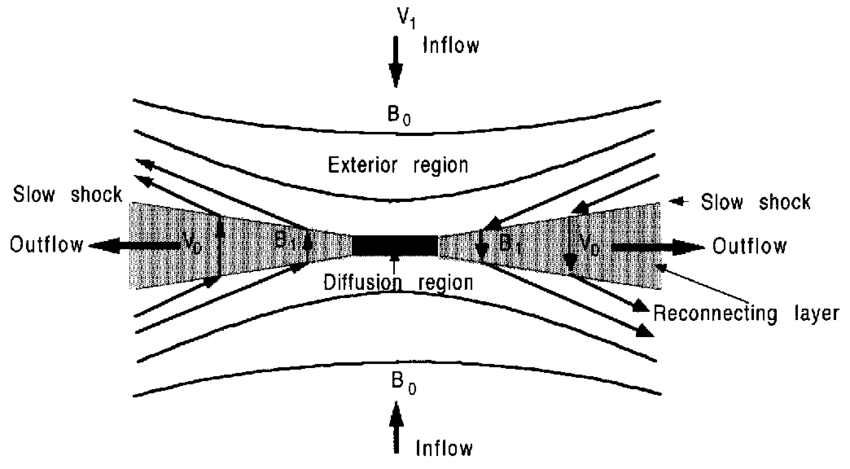
\includegraphics[width=0.45\textwidth]{petschek.png}
% 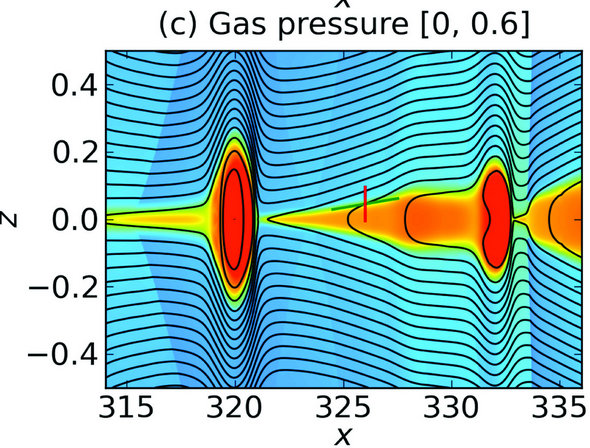
\includegraphics[width=0.4\textwidth]{shibyama.png} 
% \end{frame}

\begin{frame}{Shocks in the Universe}
%\begin{columns}
%\begin{column}{0.4\textwidth}
%\includegraphics[width=0.32\linewidth]{Figures/Crab_Nebula.jpeg}
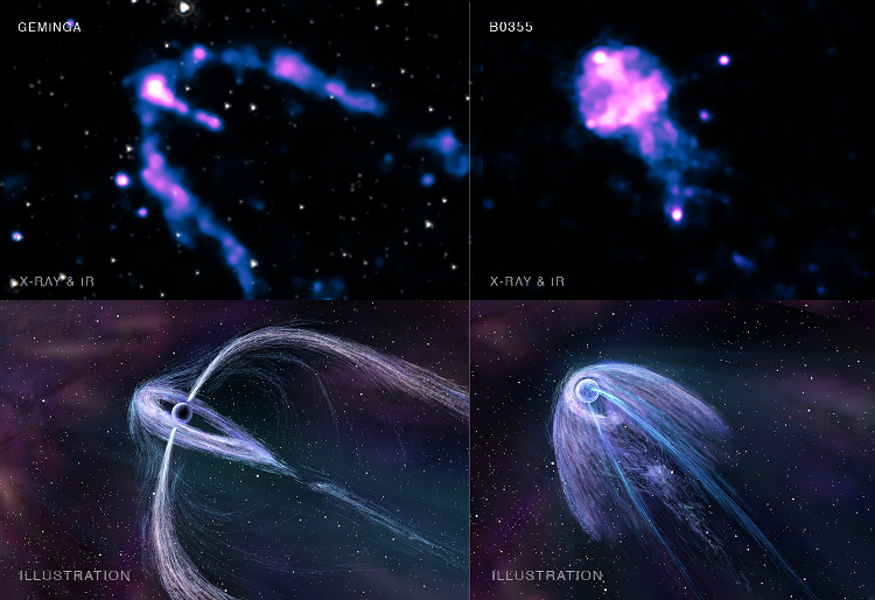
\includegraphics[width=0.32\linewidth]{Figures/pulsarwinds_chandra.jpg}
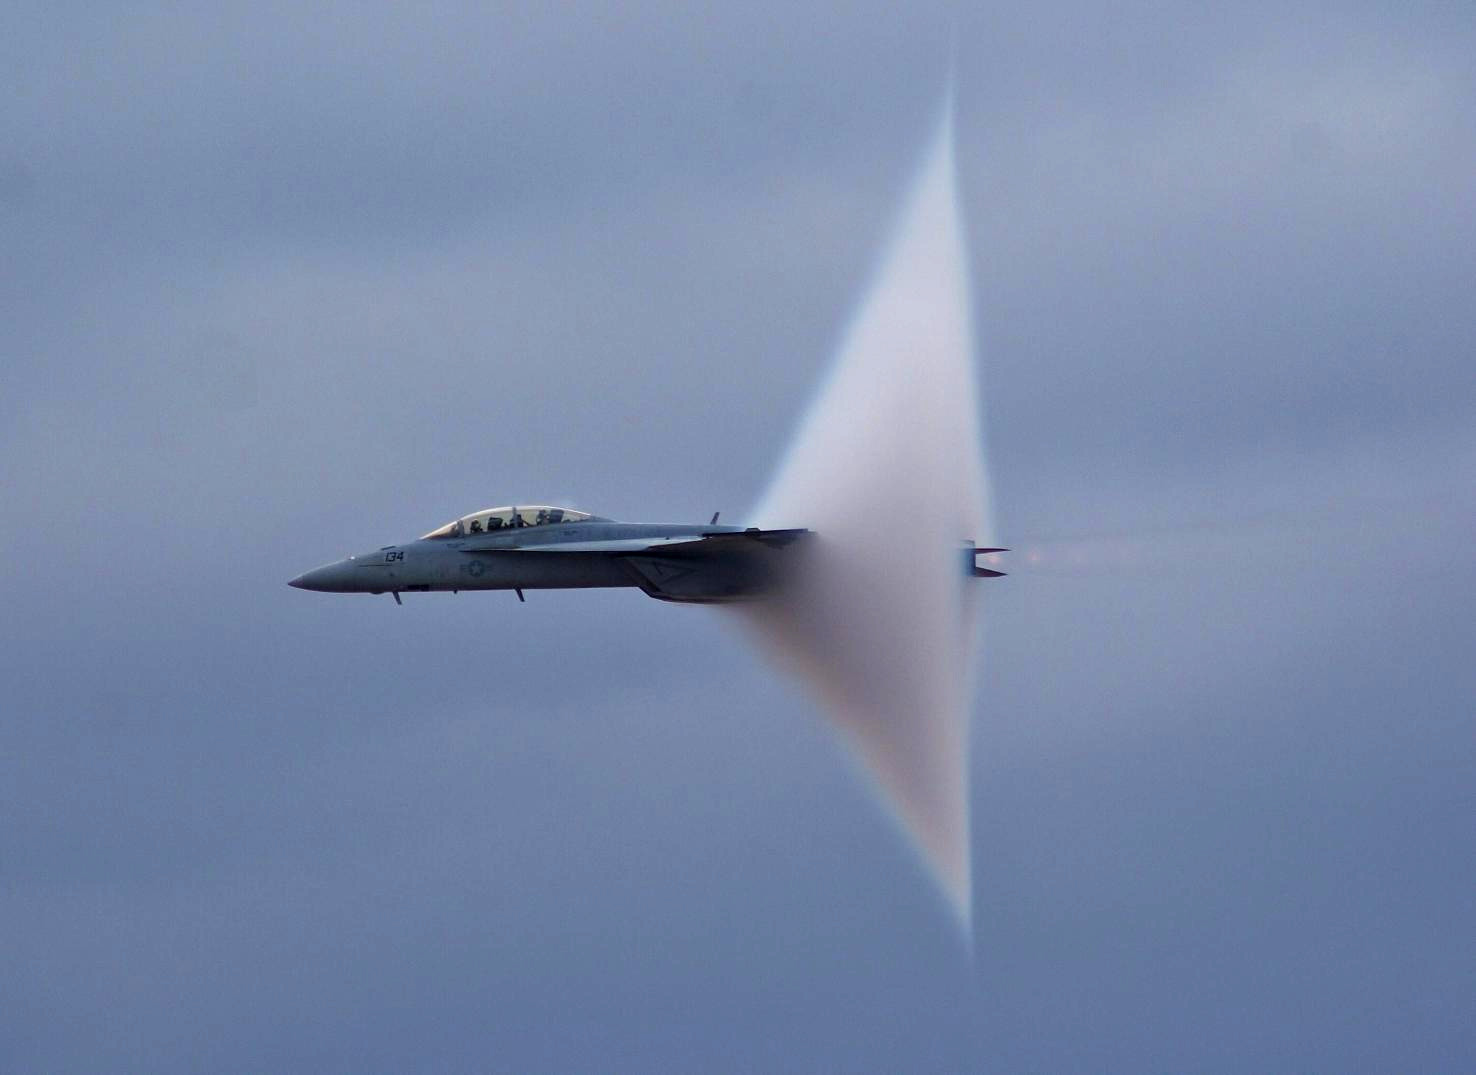
\includegraphics[width=0.32\linewidth]{Figures/FA-18_going_transonic.jpeg}
% \begin{itemize}
%     \item Shocks are universal structures
% %    \item Substructure possible.
% \end{itemize}
%\includegraphics[width=1.0\textwidth,clip=true,trim=1.0cm 1.0cm 1.0cm 1.0cm]{obs_shockloc_contour.png}
%\end{column}
%\begin{column}{0.4\textwidth}
%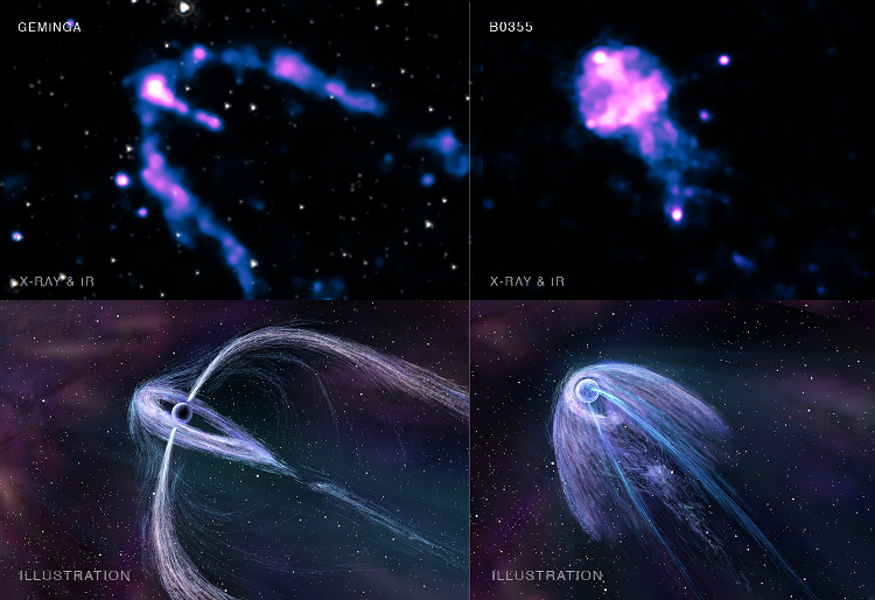
\includegraphics[width=0.95\linewidth]{Figures/pulsarwinds_chandra.jpg}
%\includegraphics[width=0.32\linewidth]{Figures/sunreconnection.jpg}
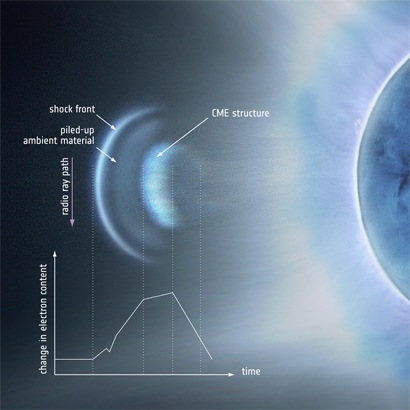
\includegraphics[width=0.32\linewidth]{Figures/cmesketch.jpg}
%\end{column}
%\end{columns}
\end{frame}

\begin{frame}{What is a shock?}
\begin{columns}
\begin{column}{0.3\textwidth}
\begin{itemize}
    \item Velocity jumps across a characteristic speed
    \item Jump in parameters
    \item Highly compressible features
    %\item Can drive turbulence
    \item Important for heating -adiabatic compression leads to temperature increases
    %\item Do shocks always heat?
\end{itemize}
%\includegraphics[width=1.0\textwidth,clip=true,trim=1.0cm 1.0cm 1.0cm 1.0cm]{obs_shockloc_contour.png}
\end{column}
\begin{column}{0.7\textwidth}
\includegraphics[width=0.95\linewidth]{Figures/shockex.jpg}
\end{column}
\end{columns}
\end{frame}

\begin{frame}{Shocks in the chromosphere}
\begin{columns}
\begin{column}{0.3\textwidth}
\begin{itemize}
    \item Solar chromosphere rife with shocks.
    \item Strong radiative losses 
    \item Solar chromosphere is partially ionised (consists of HD and MHD fluids).
    \item \textbf{Do partially ionised shocks always heat the chromosphere?}.
%    \item Substructure possible.
\end{itemize}
%\includegraphics[width=1.0\textwidth,clip=true,trim=1.0cm 1.0cm 1.0cm 1.0cm]{obs_shockloc_contour.png}
\end{column}
\begin{column}{0.7\textwidth}
\includegraphics[width=0.45\linewidth]{Figures/spicules.png}
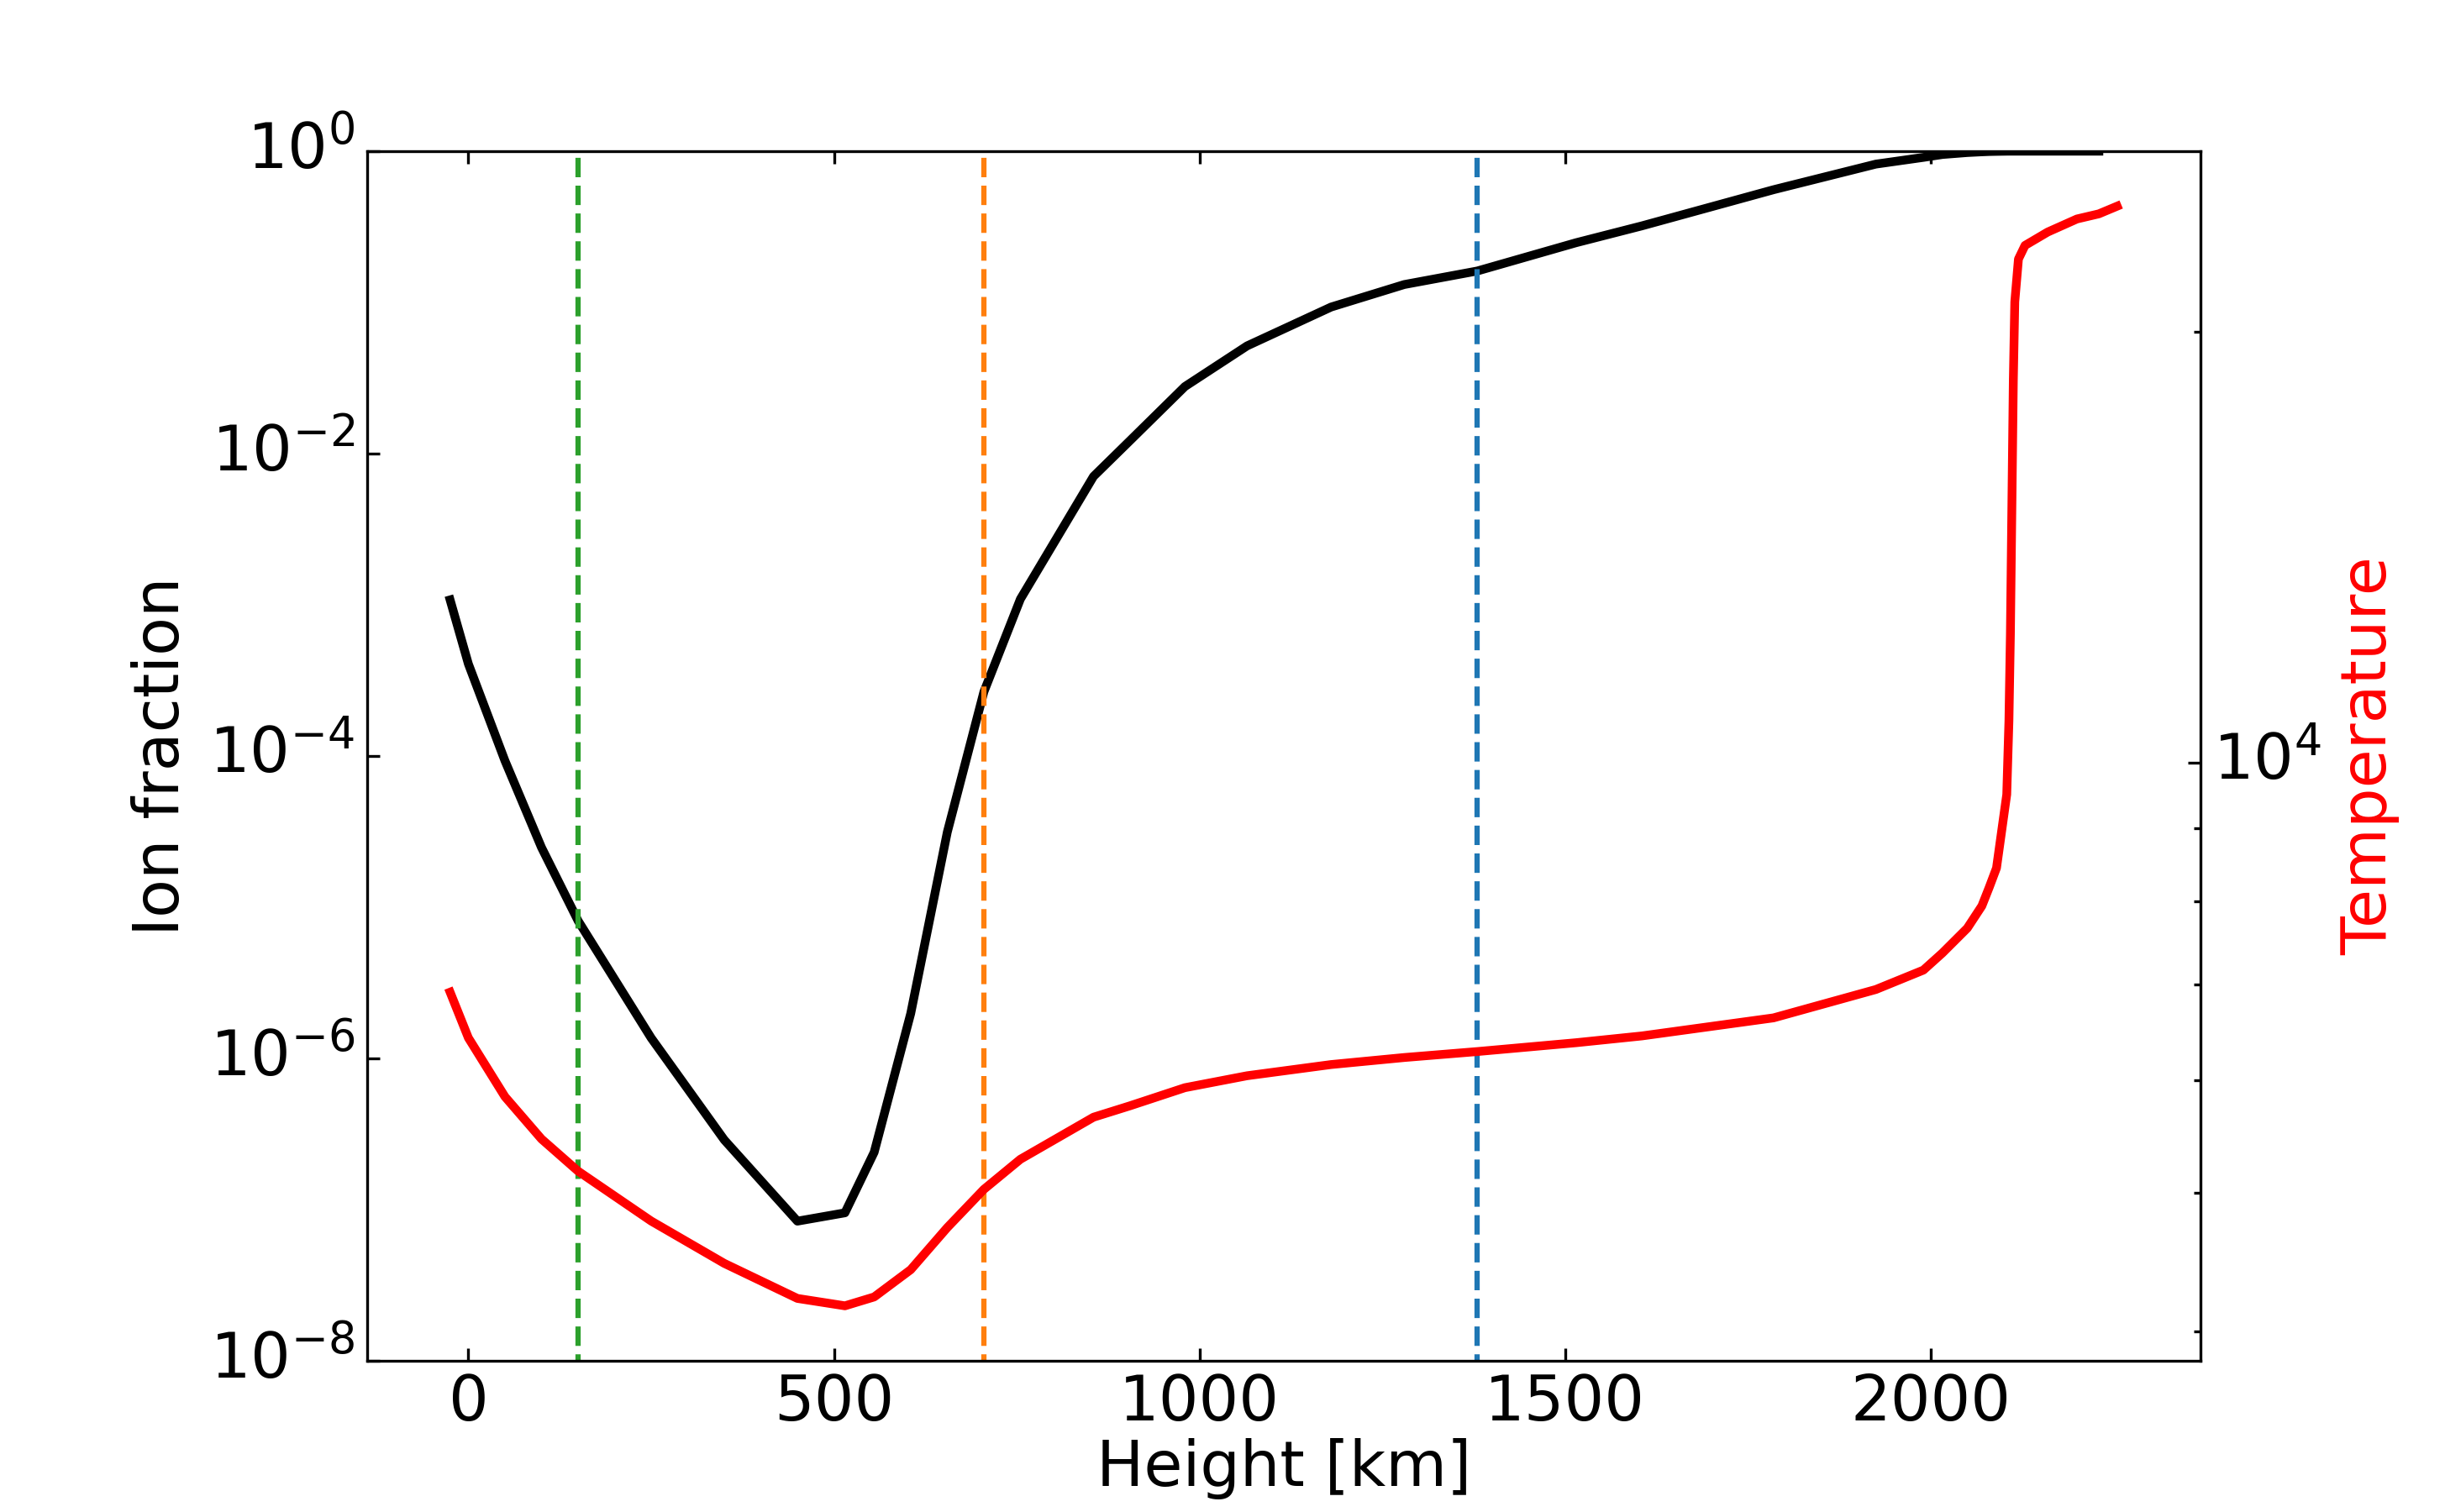
\includegraphics[width=0.5\linewidth]{Figures/saha2_plot.png}\\
\includegraphics[width=0.95\linewidth]{Figures/chromosphere.png}
\end{column}
\end{columns}
\end{frame}

\begin{frame}{Aims}
\begin{itemize}
    \item How do shocks affect temperature in HD and MHD systems?
    \item How does temperature change across a partially ionised shock?
    %\item What happens inside a partially-ionised shock?
    \item Role of shocks in heating the solar atmosphere?
\end{itemize}
\end{frame}

%%%%%%%%%%%%%%%%%%%%%%%%%%%%%%%%%%%%%%%%%%%%%%%%%%%%%%%%%%%%%%%%%%%%%%%%%%%%%%%%%%

\begin{frame}{HD shock jumps}
\begin{columns}
\begin{column}{0.4\textwidth}
\footnotesize
\begin{gather}
\frac{\partial \rho _{\text{n}}}{\partial t} + \nabla \cdot (\rho _{\text{n}} \textbf{v}_{\text{n}})= 0, \label{eqn:neutral1} \\
\frac{\partial}{\partial t}(\rho _{\text{n}} \textbf{v}_{\text{n}}) + \nabla \cdot (\rho _{\text{n}} \textbf{v}_{\text{n}} \textbf{v}_{\text{n}} + P_{\text{n}} \textbf{I}) = 0\\
\frac{\partial e_{\text{n}}}{\partial t} + \nabla \cdot \left[\textbf{v}_{\text{n}} (e_{\text{n}} +P_{\text{n}}) \right] = 0 
%e_{\text{n}} = \frac{P_{\text{n}}}{\gamma -1} + \frac{1}{2} \rho _{\text{n}} v_{\text{n}} ^2, \label{eqn:neutral2} \\
\end{gather}
Characteristic wave speed - Sound speed 
\begin{gather}
    c_s=\frac{\gamma P}{\rho}
\end{gather}
%\includegraphics[width=1.0\textwidth,clip=true,trim=1.0cm 1.0cm 1.0cm 1.0cm]{obs_shockloc_contour.png}
\end{column}
\begin{column}{0.6\textwidth}
\includegraphics[width=0.95\linewidth]{Figures/shockhd.jpg}
\end{column}
\end{columns}
\end{frame}

\begin{frame}{HD shock relations}
\begin{itemize}
    \item Jump conditions in terms of upstream Mach number $M$
\end{itemize}
\begin{gather}
    \frac{\rho_2}{\rho_1} = \frac{v_1}{v_2} = \frac{\left( \gamma +1 \right) M^2}{\left( \gamma -1 \right) M^2 +2} \\
    \frac{P_2}{P_1} = \frac{2\gamma M^2 - \left( \gamma -1\right)}{\left(\gamma +1 \right)^2M^2} \\
    \frac{T_2}{T_1} = \frac{\left[ \left( \gamma -1 \right) M^2 +2 \right] \left[ 2\gamma M^2 - \left( \gamma -1 \right) \right]}{\left(\gamma +1 \right) ^2 M^2}
\end{gather}
\begin{itemize}
    \item Temperature always increases across shock in ideal HD (kinetic energy converted to thermal energy)
\end{itemize}
\end{frame}

\begin{frame}{MHD Equations}
\begin{columns}
\begin{column}{0.45\textwidth}
\footnotesize
\begin{gather}
\frac{\partial \rho _{\text{p}}}{\partial t} + \nabla \cdot (\rho_{\text{p}} \textbf{v}_{\text{p}}) = 0 \label{eqn:plasma1}\\
\frac{\partial}{\partial t} (\rho_{\text{p}} \textbf{v}_{\text{p}})+ \nabla \cdot \left( \rho_{\text{p}} \textbf{v}_{\text{p}} \textbf{v}_{\text{p}} + P_{\text{p}} \textbf{I} - \textbf{B B} + \frac{\textbf{B}^2}{2} \textbf{I} \right) = 0\\
\frac{\partial}{\partial t} \left( e_{\text{p}} + \frac{\textbf{B}^2}{2} \right) + \nabla \cdot \left[ \textbf{v}_{\text{p}} ( e_{\text{p}} + P_{\text{p}}) -  (\textbf{v}_{\rm p} \times \textbf{B}) \times \textbf{B} \right]  =  0 \\
\frac{\partial \textbf{B}}{\partial t} - \nabla \times (\textbf{v}_{\text{p}} \times \textbf{B}) = 0.\\
%e_{\text{p}} = \frac{P_{\text{p}}}{\gamma -1} + \frac{1}{2} \rho _{\text{p}} v_{\text{p}} ^2, \\
\nabla \cdot \textbf{B} = 0,\label{eqn:plasma2}
\end{gather}
%\includegraphics[width=1.0\textwidth,clip=true,trim=1.0cm 1.0cm 1.0cm 1.0cm]{obs_shockloc_contour.png}
\end{column}
\begin{column}{0.55\textwidth}
\begin{itemize}
    \item MHD has three wave speeds: Alfv\'en, slow magnetoacoustic and fast magnetoacoustic
    \item Alfv\'en waves is purely magnetic (no associated pressure or density perturbation)
    \item Slow and fast magnetoacoustic waves are compressible and modified by the magnetic field  
\end{itemize}
\begin{gather}
    V_A=\sqrt{\frac{B^2}{\rho}}\\
    V_{f,s}=\sqrt{\frac{1}{2}\left[V_A^2+c_s^2 \pm \sqrt{\left(V_A^2 +c_s^2 \right)^2 - 4 V_A^2 c_s^2 \cos^2\theta}\right]}
\end{gather}
%\includegraphics[width=0.95\linewidth]{Figures/shockhd.jpg}
\end{column}
\end{columns}
\end{frame}


\begin{frame}{Shocks in MHD}
%\begin{columns}
%\begin{column}{0.6\textwidth}
\begin{enumerate}
\item MHD has three characteristic wave speeds (slow, Alfv\'en, fast).
%\item Multiple transitions possible.
%\item Finite shock width in two-fluid allows substructure to exist.
%\item Slow-mode shock is a transition from super-slow to sub-slow.
\item Important for reconnection, e.g., Petschek-like.
\item Intermediate shocks feature a reversal in the magnetic field across the interface.
\end{enumerate}
%\end{column}
%\begin{column}{0.5\textwidth}
%\end{column}
%\end{columns}
\begin{columns}
\begin{column}{0.5\textwidth}
\begin{itemize}
\item (1) superfast: $V_f < \abs{v_n}$,
%\item (1=2) fast: $\abs{v_n} = V_f$,
\item (2) subfast: $V_A < \abs{v_n} < V_f $,
%\item (2=3) Alfv\'en: $\abs{v_n} = V_A$,
\item (3) superslow: $V_s < \abs{v_n} < V_A$,
%\item (3=4) slow: $V_s = \abs{v_n}$,
\item (4) subslow: $0< \abs{v_n} < V_s$,
\item ($\infty$) static: $v_n = 0$.
\end{itemize}
\end{column}
\begin{column}{0.5\textwidth}
\begin{itemize}
\item $1 \rightarrow 2 $ fast shocks
\item $3 \rightarrow 4$ slow shocks
%\item $1 \rightarrow 2=3$ switch-on
%\item $2=3 \rightarrow 4$ switch-off
\item $1\rightarrow 3, 1 \rightarrow 4, 2 \rightarrow 3, 2 \rightarrow 4$ intermediate shocks
\end{itemize}
\end{column}
\end{columns}
\end{frame}

\begin{frame}{MHD shock jumps}
\begin{columns}
\begin{column}{0.45\textwidth}
\begin{gather}
    \left[\rho v_x  \right]^u _d = 0,  \\
    \left[\rho v_x^2 +P +\frac{B_y^2}{2} \right]^u _d = 0, \\
    \left[\rho v_x v_y -B_x B_y \right]^u _d = 0, \\
    \left[ v_{x} \left( \frac{\gamma}{\gamma -1} P + \frac{1}{2} \rho v^2 \right) \right]^u _d =0, \\
    \left[B_x \right]^u _d = 0, \\
    \left[v_x B_y -v_y B_x   \right]^u _d = 0, 
\end{gather}
where
\begin{gather}
    \left[ Q \right]^u _d \equiv Q^u - Q^d,
\end{gather}
\end{column}
\begin{column}{0.55\textwidth}
\footnotesize
\begin{itemize}
    \item Analytical solution exists for MHD shock jump equations exists (Hau \& Sonnerup 1989) 
\end{itemize}
\begin{gather}
    A_x ^{\text{u}2} = \left[ A_x ^{\text{d}2} \left( \frac{\gamma-1}{\gamma} \left( \frac{\gamma+1}{\gamma -1} -\tan ^2 \theta \right) \left(A_x ^{\text{d}2} -1 \right) ^2 \right. \right. \nonumber\\ 
    + \left. \left. \tan ^2 \theta \left( \frac{\gamma-1}{\gamma} A_x ^{\text{d}2} -1 \right) \left(A_x ^{\text{d}2} -2 \right) \right) - \frac{\beta}{ \cos ^2 \theta } \left( A_x ^{\text{d}2} -1 \right) ^2 \right]  \nonumber\\
    / \left[ \frac{\gamma -1}{\gamma} \frac{\left( A_x ^{\text{d}2}-1 \right) ^2}{ \cos ^2 \theta } - A_ x ^{\text{d}2} \tan ^2 \theta \left( \frac{\gamma -1}{\gamma} A_x ^{\text{d}2} -1 \right) \right].
\end{gather}
In the MHD model, there is a limitation on the compressionality of the system that arises from the energy equation, namely 
\begin{gather}
    1 \leq r \leq \frac{\gamma +1}{\gamma -1}.
\end{gather}
For $\gamma =5/3$, this leads to a maximum compression ratio of $r=4$.

\textbf{Temperature increases across an MHD shock}
\end{column}
\end{columns}
\end{frame}

\begin{frame}{Partial ionisation - overview}
\begin{columns}
\begin{column}{0.4\textwidth}
\begin{itemize}
    % \item Solar chromosphere is partially ionised.
    % \item Understanding two-fluid shocks is fundamental to understanding energy transfer and heating in the solar chromosphere and corona.
    \item Neutral hydrogen follows hydrodynamic equations
    \item Ionised hydrogen follows MHD equations
    \item Partially-ionised systems consist of both HD and MHD systems that interact.
    \item Examples: solar chromosphere, interstellar medium, lab plasmas...
%    \item Substructure possible.
\end{itemize}
%\includegraphics[width=1.0\textwidth,clip=true,trim=1.0cm 1.0cm 1.0cm 1.0cm]{obs_shockloc_contour.png}
\end{column}
\begin{column}{0.6\textwidth}
\includegraphics[width=0.95\linewidth]{Figures/hydrogensketch.png} 
\end{column}
\end{columns}
\end{frame}

\begin{frame}{Two-fluid shocks - overview}
\begin{columns}
\begin{column}{0.4\textwidth}
\begin{itemize}
    % \item Solar chromosphere is partially ionised.
    % \item Understanding two-fluid shocks is fundamental to understanding energy transfer and heating in the solar chromosphere and corona.
    \item Two-fluid shocks have a finite width as opposed to the discontinuous single-fluid MHD case.
    \item Same overall shock jump but substructure exists.
    \item Ionisation/recombination rates increased in shocks - needs to be considered.
%    \item Substructure possible.
\end{itemize}
%\includegraphics[width=1.0\textwidth,clip=true,trim=1.0cm 1.0cm 1.0cm 1.0cm]{obs_shockloc_contour.png}
\end{column}
\begin{column}{0.6\textwidth}
%\includegraphics[width=0.95\linewidth,clip=true,trim=0.9cm 7.8cm 1.5cm 7.8cm]{poster_comp.pdf} \\
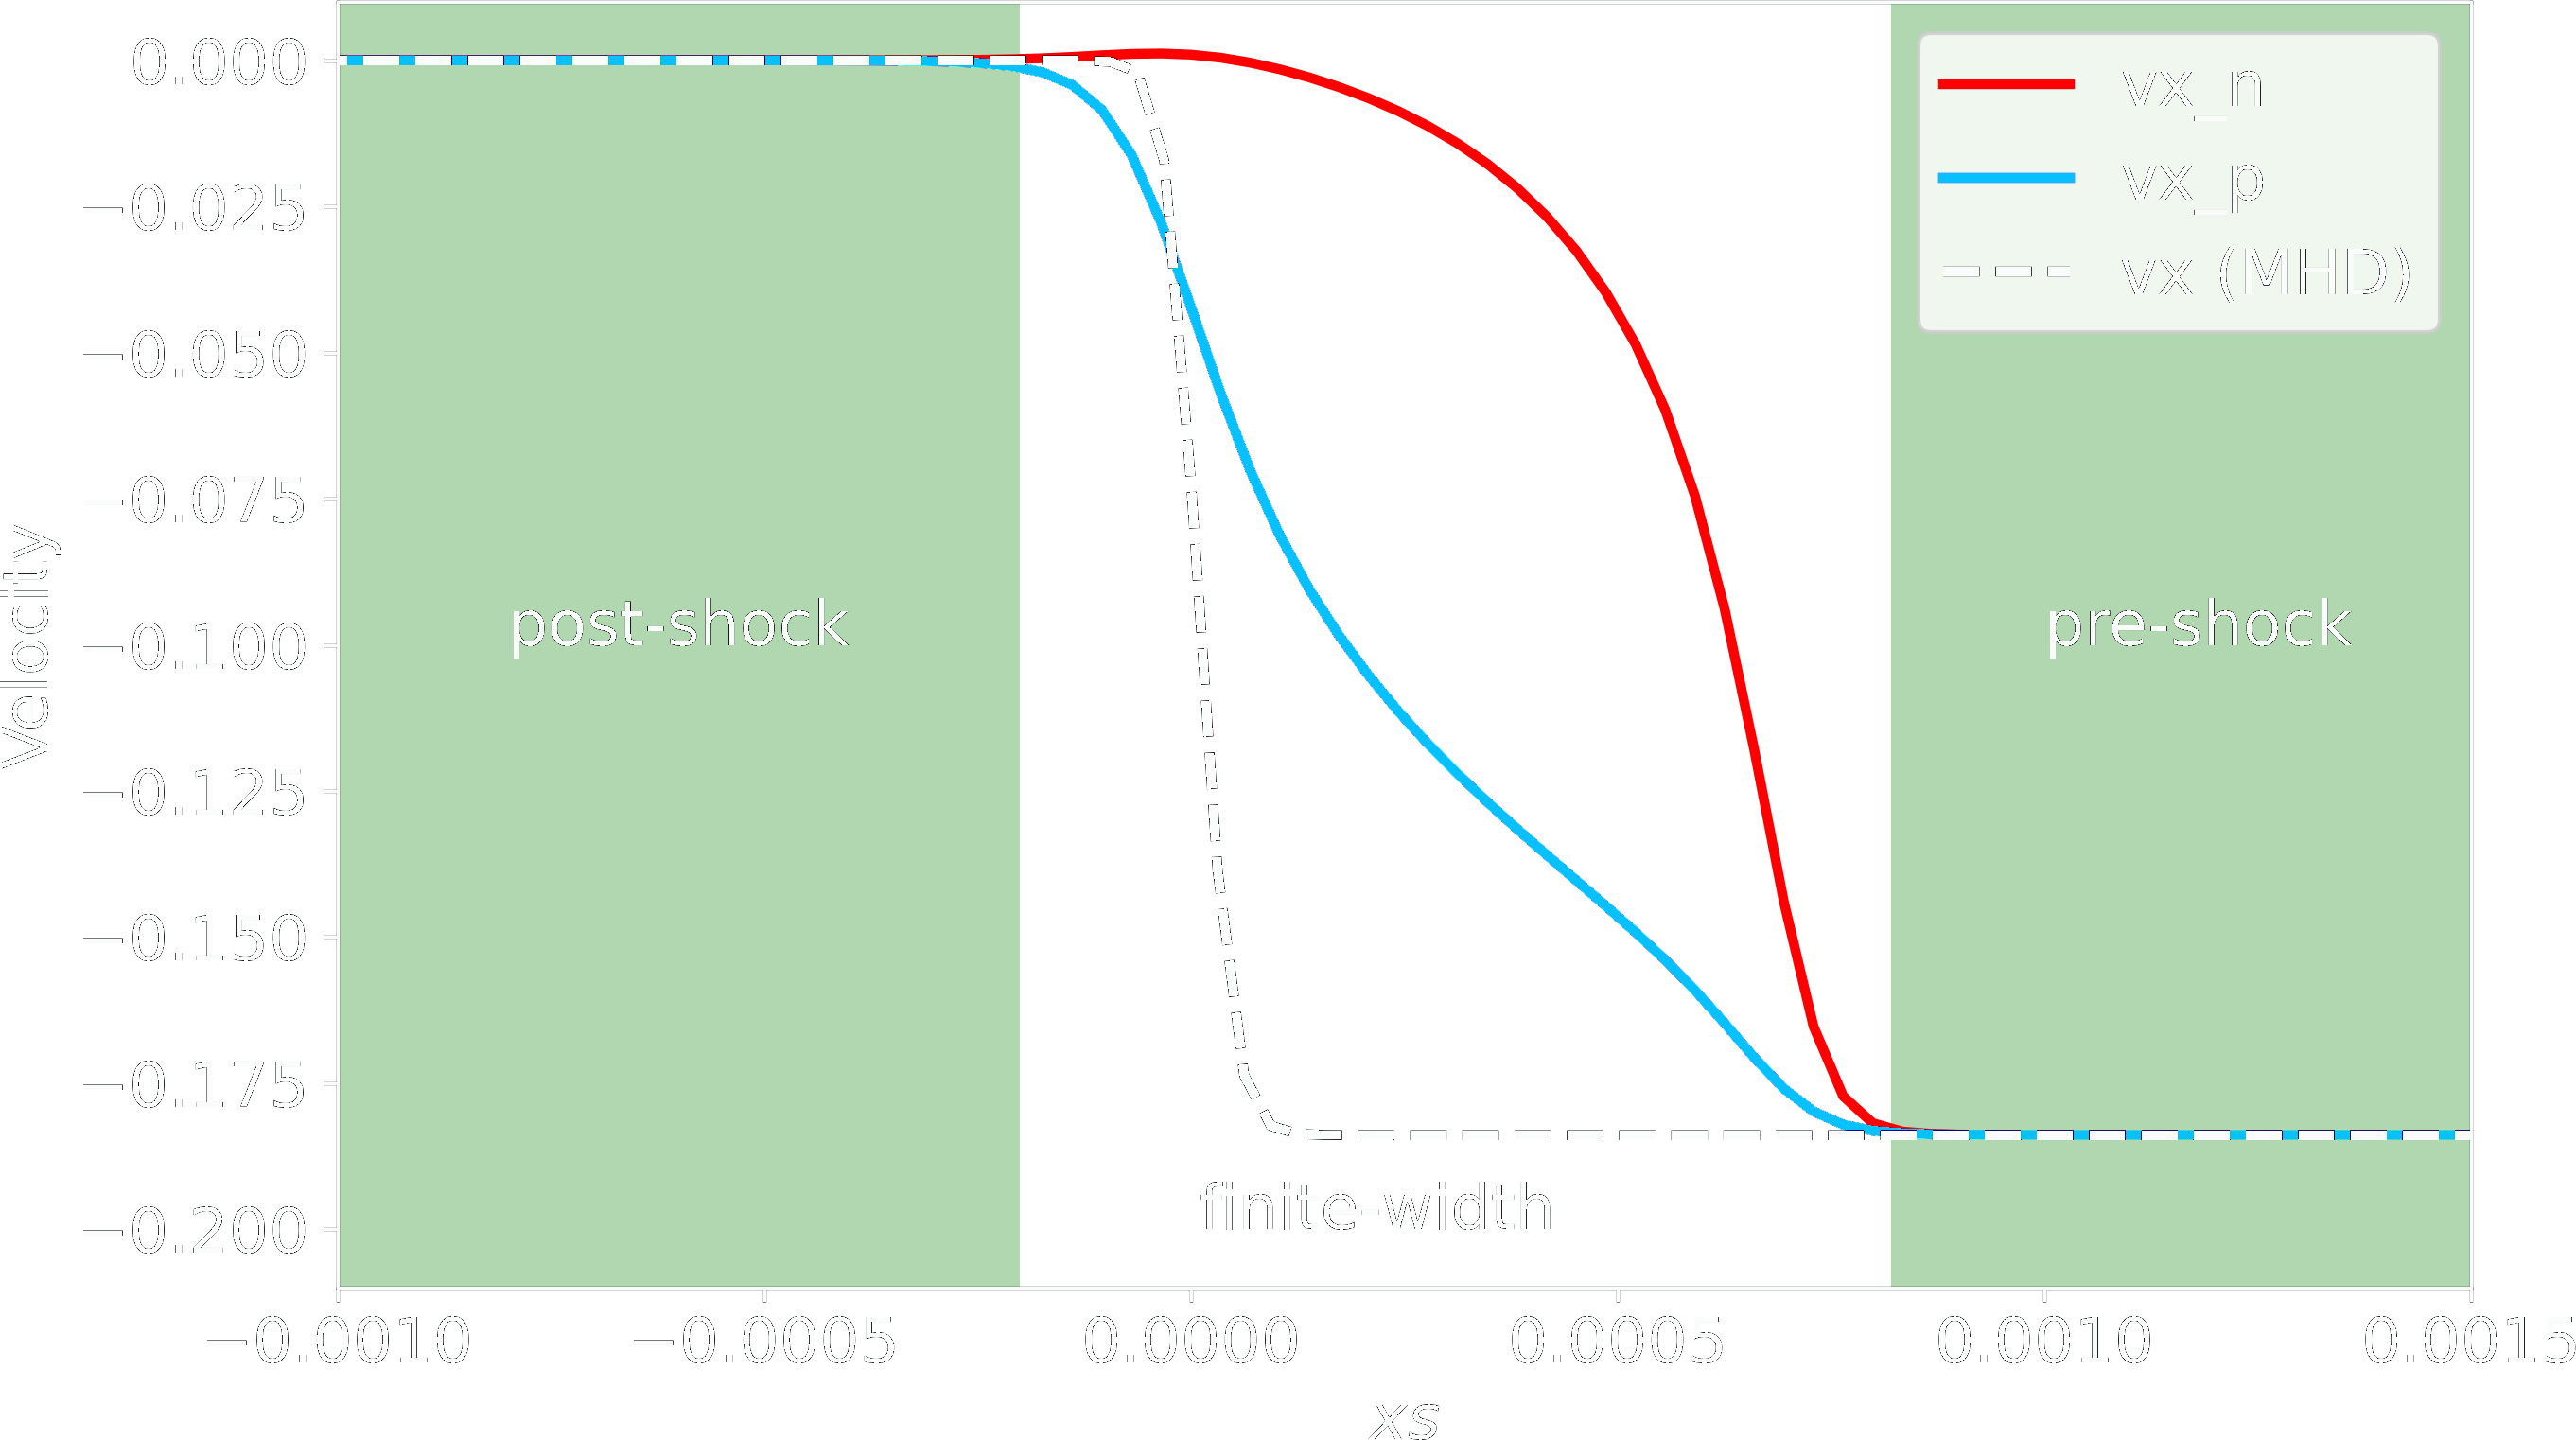
\includegraphics[width=0.95\linewidth]{Figures/shocksub_col.png} \\
Conservative equations (e.g., two-fluid with thermal collisions) leads to MHD shock jumps, Snow \& Hillier 2019.
\end{column}
\end{columns}
\end{frame}

\begin{frame}{Ionisation, recombination and ionisation potential in two-fluid shocks}
\footnotesize
\begin{gather}
\frac{\partial \rho _{\text{n}}}{\partial t} + \nabla \cdot (\rho _{\text{n}} \textbf{v}_{\text{n}})= \Gamma _{rec} \rho _{\rm p} - \Gamma _{ion} \rho _{\rm n}, \label{eqn:neutral1}\tag{5} \\
\frac{\partial}{\partial t}(\rho _{\text{n}} \textbf{v}_{\text{n}}) + \nabla \cdot (\rho _{\text{n}} \textbf{v}_{\text{n}} \textbf{v}_{\text{n}} + P_{\text{n}} \textbf{I}) = -\alpha _c \rho_{\text{n}} \rho_{\text{p}} (\textbf{v}_{\text{n}}-\textbf{v}_{\text{p}}) + \Gamma _{rec} \rho _{\rm p} \textbf{v}_{\rm p} - \Gamma _{ion} \rho_{\rm n} \textbf{v}_{\rm n}, \tag{6}\\
\frac{\partial e_{\text{n}}}{\partial t} + \nabla \cdot \left[\textbf{v}_{\text{n}} (e_{\text{n}} +P_{\text{n}}) \right] = -\alpha _c \rho _{\text{n}} \rho _{\text{p}} \left[ \frac{1}{2} (\textbf{v}_{\text{n}} ^2 - \textbf{v}_{\text{p}} ^2)+ \frac{3}{2} \left(\frac{P_{\rm n}}{\rho_{\rm n}}-\frac{1}{2}\frac{P_{\rm p}}{\rho_{\rm p}}\right) \right] \nonumber \\ \hspace{0.5cm}+ \frac{1}{2} \left( \Gamma _{rec} \rho _{\rm p} \textbf{v}_{\rm p} ^2 - \Gamma _{ion} \rho _{\rm n} \textbf{v}_{\rm n} ^2 \right) +\frac{1}{ (\gamma-1)} \left( \frac{1}{2} \Gamma _{rec} P_{\rm p} -\Gamma _{ion} P_{\rm n} \right), \tag{7}\\
%e_{\text{n}} = \frac{P_{\text{n}}}{\gamma -1} + \frac{1}{2} \rho _{\text{n}} v_{\text{n}} ^2, \label{eqn:neutral2} \\
\frac{\partial \rho _{\text{p}}}{\partial t} + \nabla \cdot (\rho_{\text{p}} \textbf{v}_{\text{p}}) = - \Gamma _{rec} \rho _{\rm p} + \Gamma _{ion} \rho _{\rm n} \label{eqn:plasma1}\tag{8}\\
\frac{\partial}{\partial t} (\rho_{\text{p}} \textbf{v}_{\text{p}})+ \nabla \cdot \left( \rho_{\text{p}} \textbf{v}_{\text{p}} \textbf{v}_{\text{p}} + P_{\text{p}} \textbf{I} - \textbf{B B} + \frac{\textbf{B}^2}{2} \textbf{I} \right) = \alpha _c \rho_{\text{n}} \rho_{\text{p}}(\textbf{v}_{\text{n}} - \textbf{v}_{\text{p}}) - \Gamma _{rec} \rho _{\rm p} \textbf{v}_{\rm p} + \Gamma _{ion} \rho_{\rm n} \textbf{v}_{\rm n},\tag{9}\\
\frac{\partial}{\partial t} \left( e_{\text{p}} + \frac{\textbf{B}^2}{2} \right) + \nabla \cdot \left[ \textbf{v}_{\text{p}} ( e_{\text{p}} + P_{\text{p}}) -  (\textbf{v}_{\rm p} \times \textbf{B}) \times \textbf{B} \right]  =  \alpha _c \rho _{\text{n}} \rho _{\text{p}} \left[ \frac{1}{2} (\textbf{v}_{\text{n}} ^2 - \textbf{v}_{\text{p}} ^2)+ \frac{3}{2} \left(\frac{P_{\rm n}}{\rho_{\rm n}}-\frac{1}{2}\frac{P_{\rm p}}{\rho_{\rm p}}\right) \right] \nonumber \\ \hspace{0.5cm}- \frac{1}{2} \left( \Gamma _{rec} \rho _{\rm p} \textbf{v}_{\rm p} ^2 - \Gamma _{ion} \rho _{\rm n} \textbf{v}_{\rm n} ^2 \right) {- \phi_I + A_{heat}} -\frac{1}{ (\gamma-1)} \left( \frac{1}{2} \Gamma _{rec} P_{\rm p} -\Gamma _{ion} P_{\rm n} \right), \label{eqn:ep}\tag{10} \\
\frac{\partial \textbf{B}}{\partial t} - \nabla \times (\textbf{v}_{\text{p}} \times \textbf{B}) = 0.\tag{11}
%e_{\text{p}} = \frac{P_{\text{p}}}{\gamma -1} + \frac{1}{2} \rho _{\text{p}} v_{\text{p}} ^2, \\
%\nabla \cdot \textbf{B} = 0,\label{eqn:plasma2}
\end{gather}
\end{frame}

\begin{frame}{Ionisation, recombination and ionisation potential in two-fluid shocks}
\vspace{-0.5cm}
\footnotesize
\begin{gather}
\mathcolorbox{VioletRed}{\frac{\partial \rho _{\text{n}}}{\partial t} + \nabla \cdot (\rho _{\text{n}} \textbf{v}_{\text{n}})}= \Gamma _{rec} \rho _{\rm p} - \Gamma _{ion} \rho _{\rm n}, \label{eqn:neutral1}\tag{5} \\
\mathcolorbox{VioletRed}{\frac{\partial}{\partial t}(\rho _{\text{n}} \textbf{v}_{\text{n}}) + \nabla \cdot (\rho _{\text{n}} \textbf{v}_{\text{n}} \textbf{v}_{\text{n}} + P_{\text{n}} \textbf{I})} = -\alpha _c \rho_{\text{n}} \rho_{\text{p}} (\textbf{v}_{\text{n}}-\textbf{v}_{\text{p}}) + \Gamma _{rec} \rho _{\rm p} \textbf{v}_{\rm p} - \Gamma _{ion} \rho_{\rm n} \textbf{v}_{\rm n}, \tag{6}\\
\mathcolorbox{VioletRed}{\frac{\partial e_{\text{n}}}{\partial t} + \nabla \cdot \left[\textbf{v}_{\text{n}} (e_{\text{n}} +P_{\text{n}}) \right]} = -\alpha _c \rho _{\text{n}} \rho _{\text{p}} \left[ \frac{1}{2} (\textbf{v}_{\text{n}} ^2 - \textbf{v}_{\text{p}} ^2)+ \frac{3}{2} \left(\frac{P_{\rm n}}{\rho_{\rm n}}-\frac{1}{2}\frac{P_{\rm p}}{\rho_{\rm p}}\right) \right] \nonumber \\ \hspace{0.5cm}+ \frac{1}{2} \left( \Gamma _{rec} \rho _{\rm p} \textbf{v}_{\rm p} ^2 - \Gamma _{ion} \rho _{\rm n} \textbf{v}_{\rm n} ^2 \right) +\frac{1}{ (\gamma-1)} \left( \frac{1}{2} \Gamma _{rec} P_{\rm p} -\Gamma _{ion} P_{\rm n} \right), \tag{7}\\
%e_{\text{n}} = \frac{P_{\text{n}}}{\gamma -1} + \frac{1}{2} \rho _{\text{n}} v_{\text{n}} ^2, \label{eqn:neutral2} \\
\frac{\partial \rho _{\text{p}}}{\partial t} + \nabla \cdot (\rho_{\text{p}} \textbf{v}_{\text{p}}) = - \Gamma _{rec} \rho _{\rm p} + \Gamma _{ion} \rho _{\rm n} \label{eqn:plasma1}\tag{8}\\
\frac{\partial}{\partial t} (\rho_{\text{p}} \textbf{v}_{\text{p}})+ \nabla \cdot \left( \rho_{\text{p}} \textbf{v}_{\text{p}} \textbf{v}_{\text{p}} + P_{\text{p}} \textbf{I} - \textbf{B B} + \frac{\textbf{B}^2}{2} \textbf{I} \right) = \alpha _c \rho_{\text{n}} \rho_{\text{p}}(\textbf{v}_{\text{n}} - \textbf{v}_{\text{p}}) - \Gamma _{rec} \rho _{\rm p} \textbf{v}_{\rm p} + \Gamma _{ion} \rho_{\rm n} \textbf{v}_{\rm n},\tag{9}\\
\frac{\partial}{\partial t} \left( e_{\text{p}} + \frac{\textbf{B}^2}{2} \right) + \nabla \cdot \left[ \textbf{v}_{\text{p}} ( e_{\text{p}} + P_{\text{p}}) -  (\textbf{v}_{\rm p} \times \textbf{B}) \times \textbf{B} \right]  =  \alpha _c \rho _{\text{n}} \rho _{\text{p}} \left[ \frac{1}{2} (\textbf{v}_{\text{n}} ^2 - \textbf{v}_{\text{p}} ^2)+ \frac{3}{2} \left(\frac{P_{\rm n}}{\rho_{\rm n}}-\frac{1}{2}\frac{P_{\rm p}}{\rho_{\rm p}}\right) \right] \nonumber \\ \hspace{0.5cm}- \frac{1}{2} \left( \Gamma _{rec} \rho _{\rm p} \textbf{v}_{\rm p} ^2 - \Gamma _{ion} \rho _{\rm n} \textbf{v}_{\rm n} ^2 \right) {- \phi_I + A_{heat}} -\frac{1}{ (\gamma-1)} \left( \frac{1}{2} \Gamma _{rec} P_{\rm p} -\Gamma _{ion} P_{\rm n} \right), \label{eqn:ep} \tag{10}\\
\frac{\partial \textbf{B}}{\partial t} - \nabla \times (\textbf{v}_{\text{p}} \times \textbf{B}) = 0.\tag{11}
%e_{\text{p}} = \frac{P_{\text{p}}}{\gamma -1} + \frac{1}{2} \rho _{\text{p}} v_{\text{p}} ^2, \\
%\nabla \cdot \textbf{B} = 0,\label{eqn:plasma2}
\end{gather}
\end{frame}

\begin{frame}{Ionisation, recombination and ionisation potential in two-fluid shocks}
\vspace{-0.5cm}
\footnotesize
\begin{gather}
\frac{\partial \rho _{\text{n}}}{\partial t} + \nabla \cdot (\rho _{\text{n}} \textbf{v}_{\text{n}})= \Gamma _{rec} \rho _{\rm p} - \Gamma _{ion} \rho _{\rm n}, \label{eqn:neutral1}\tag{5} \\
\frac{\partial}{\partial t}(\rho _{\text{n}} \textbf{v}_{\text{n}}) + \nabla \cdot (\rho _{\text{n}} \textbf{v}_{\text{n}} \textbf{v}_{\text{n}} + P_{\text{n}} \textbf{I}) = -\alpha _c \rho_{\text{n}} \rho_{\text{p}} (\textbf{v}_{\text{n}}-\textbf{v}_{\text{p}}) + \Gamma _{rec} \rho _{\rm p} \textbf{v}_{\rm p} - \Gamma _{ion} \rho_{\rm n} \textbf{v}_{\rm n}, \tag{6}\\
\frac{\partial e_{\text{n}}}{\partial t} + \nabla \cdot \left[\textbf{v}_{\text{n}} (e_{\text{n}} +P_{\text{n}}) \right] = -\alpha _c \rho _{\text{n}} \rho _{\text{p}} \left[ \frac{1}{2} (\textbf{v}_{\text{n}} ^2 - \textbf{v}_{\text{p}} ^2)+ \frac{3}{2} \left(\frac{P_{\rm n}}{\rho_{\rm n}}-\frac{1}{2}\frac{P_{\rm p}}{\rho_{\rm p}}\right) \right] \nonumber \\ \hspace{0.5cm}+ \frac{1}{2} \left( \Gamma _{rec} \rho _{\rm p} \textbf{v}_{\rm p} ^2 - \Gamma _{ion} \rho _{\rm n} \textbf{v}_{\rm n} ^2 \right) +\frac{1}{ (\gamma-1)} \left( \frac{1}{2} \Gamma _{rec} P_{\rm p} -\Gamma _{ion} P_{\rm n} \right), \tag{7}\\
%e_{\text{n}} = \frac{P_{\text{n}}}{\gamma -1} + \frac{1}{2} \rho _{\text{n}} v_{\text{n}} ^2, \label{eqn:neutral2} \\
\mathcolorbox{BlueGreen}{\frac{\partial \rho _{\text{p}}}{\partial t} + \nabla \cdot (\rho_{\text{p}} \textbf{v}_{\text{p}})} = - \Gamma _{rec} \rho _{\rm p} + \Gamma _{ion} \rho _{\rm n} \label{eqn:plasma1}\tag{8}\\
\mathcolorbox{BlueGreen}{\frac{\partial}{\partial t} (\rho_{\text{p}} \textbf{v}_{\text{p}})+ \nabla \cdot \left( \rho_{\text{p}} \textbf{v}_{\text{p}} \textbf{v}_{\text{p}} + P_{\text{p}} \textbf{I} - \textbf{B B} + \frac{\textbf{B}^2}{2} \textbf{I} \right)} = \alpha _c \rho_{\text{n}} \rho_{\text{p}}(\textbf{v}_{\text{n}} - \textbf{v}_{\text{p}}) - \Gamma _{rec} \rho _{\rm p} \textbf{v}_{\rm p} + \Gamma _{ion} \rho_{\rm n} \textbf{v}_{\rm n},\tag{9}\\
\mathcolorbox{BlueGreen}{\frac{\partial}{\partial t} \left( e_{\text{p}} + \frac{\textbf{B}^2}{2} \right) + \nabla \cdot \left[ \textbf{v}_{\text{p}} ( e_{\text{p}} + P_{\text{p}}) -  (\textbf{v}_{\rm p} \times \textbf{B}) \times \textbf{B} \right] } =  \alpha _c \rho _{\text{n}} \rho _{\text{p}} \left[ \frac{1}{2} (\textbf{v}_{\text{n}} ^2 - \textbf{v}_{\text{p}} ^2)+ \frac{3}{2} \left(\frac{P_{\rm n}}{\rho_{\rm n}}-\frac{1}{2}\frac{P_{\rm p}}{\rho_{\rm p}}\right) \right] \nonumber \\ \hspace{0.5cm}- \frac{1}{2} \left( \Gamma _{rec} \rho _{\rm p} \textbf{v}_{\rm p} ^2 - \Gamma _{ion} \rho _{\rm n} \textbf{v}_{\rm n} ^2 \right) {- \phi_I + A_{heat}} -\frac{1}{ (\gamma-1)} \left( \frac{1}{2} \Gamma _{rec} P_{\rm p} -\Gamma _{ion} P_{\rm n} \right), \label{eqn:ep}\tag{10} \\
\mathcolorbox{BlueGreen}{\frac{\partial \textbf{B}}{\partial t} - \nabla \times (\textbf{v}_{\text{p}} \times \textbf{B}) = 0.}\tag{11}
%e_{\text{p}} = \frac{P_{\text{p}}}{\gamma -1} + \frac{1}{2} \rho _{\text{p}} v_{\text{p}} ^2, \\
%\nabla \cdot \textbf{B} = 0,\label{eqn:plasma2}
\end{gather}
\end{frame}

\begin{frame}{Ionisation, recombination and ionisation potential in two-fluid shocks}
\vspace{-0.5cm}
\footnotesize
\begin{gather}
\frac{\partial \rho _{\text{n}}}{\partial t} + \nabla \cdot (\rho _{\text{n}} \textbf{v}_{\text{n}})= \Gamma _{rec} \rho _{\rm p} - \Gamma _{ion} \rho _{\rm n}, \label{eqn:neutral1}\tag{5} \\
\frac{\partial}{\partial t}(\rho _{\text{n}} \textbf{v}_{\text{n}}) + \nabla \cdot (\rho _{\text{n}} \textbf{v}_{\text{n}} \textbf{v}_{\text{n}} + P_{\text{n}} \textbf{I}) =\mathcolorbox{YellowOrange}{ -\alpha _c \rho_{\text{n}} \rho_{\text{p}} (\textbf{v}_{\text{n}}-\textbf{v}_{\text{p}})} + \Gamma _{rec} \rho _{\rm p} \textbf{v}_{\rm p} - \Gamma _{ion} \rho_{\rm n} \textbf{v}_{\rm n}, \tag{6}\\
\frac{\partial e_{\text{n}}}{\partial t} + \nabla \cdot \left[\textbf{v}_{\text{n}} (e_{\text{n}} +P_{\text{n}}) \right] = \mathcolorbox{YellowOrange}{-\alpha _c \rho _{\text{n}} \rho _{\text{p}} \left[ \frac{1}{2} (\textbf{v}_{\text{n}} ^2 - \textbf{v}_{\text{p}} ^2)+ \frac{3}{2} \left(\frac{P_{\rm n}}{\rho_{\rm n}}-\frac{1}{2}\frac{P_{\rm p}}{\rho_{\rm p}}\right) \right]} \nonumber \\ \hspace{0.5cm}+ \frac{1}{2} \left( \Gamma _{rec} \rho _{\rm p} \textbf{v}_{\rm p} ^2 - \Gamma _{ion} \rho _{\rm n} \textbf{v}_{\rm n} ^2 \right) +\frac{1}{ (\gamma-1)} \left( \frac{1}{2} \Gamma _{rec} P_{\rm p} -\Gamma _{ion} P_{\rm n} \right), \tag{7}\\
%e_{\text{n}} = \frac{P_{\text{n}}}{\gamma -1} + \frac{1}{2} \rho _{\text{n}} v_{\text{n}} ^2, \label{eqn:neutral2} \\
\frac{\partial \rho _{\text{p}}}{\partial t} + \nabla \cdot (\rho_{\text{p}} \textbf{v}_{\text{p}}) = - \Gamma _{rec} \rho _{\rm p} + \Gamma _{ion} \rho _{\rm n} \label{eqn:plasma1}\tag{8}\\
\frac{\partial}{\partial t} (\rho_{\text{p}} \textbf{v}_{\text{p}})+ \nabla \cdot \left( \rho_{\text{p}} \textbf{v}_{\text{p}} \textbf{v}_{\text{p}} + P_{\text{p}} \textbf{I} - \textbf{B B} + \frac{\textbf{B}^2}{2} \textbf{I} \right) = \mathcolorbox{YellowOrange}{\alpha _c \rho_{\text{n}} \rho_{\text{p}}(\textbf{v}_{\text{n}} - \textbf{v}_{\text{p}})} - \Gamma _{rec} \rho _{\rm p} \textbf{v}_{\rm p} + \Gamma _{ion} \rho_{\rm n} \textbf{v}_{\rm n},\tag{9}\\
\frac{\partial}{\partial t} \left( e_{\text{p}} + \frac{\textbf{B}^2}{2} \right) + \nabla \cdot \left[ \textbf{v}_{\text{p}} ( e_{\text{p}} + P_{\text{p}}) -  (\textbf{v}_{\rm p} \times \textbf{B}) \times \textbf{B} \right]  = \mathcolorbox{YellowOrange}{ \alpha _c \rho _{\text{n}} \rho _{\text{p}} \left[ \frac{1}{2} (\textbf{v}_{\text{n}} ^2 - \textbf{v}_{\text{p}} ^2)+ \frac{3}{2} \left(\frac{P_{\rm n}}{\rho_{\rm n}}-\frac{1}{2}\frac{P_{\rm p}}{\rho_{\rm p}}\right) \right]} \nonumber \\ \hspace{0.5cm}- \frac{1}{2} \left( \Gamma _{rec} \rho _{\rm p} \textbf{v}_{\rm p} ^2 - \Gamma _{ion} \rho _{\rm n} \textbf{v}_{\rm n} ^2 \right) {- \phi_I + A_{heat}} -\frac{1}{ (\gamma-1)} \left( \frac{1}{2} \Gamma _{rec} P_{\rm p} -\Gamma _{ion} P_{\rm n} \right), \label{eqn:ep} \tag{10}\\
\frac{\partial \textbf{B}}{\partial t} - \nabla \times (\textbf{v}_{\text{p}} \times \textbf{B}) = 0.\tag{11}
%e_{\text{p}} = \frac{P_{\text{p}}}{\gamma -1} + \frac{1}{2} \rho _{\text{p}} v_{\text{p}} ^2, \\
%\nabla \cdot \textbf{B} = 0,\label{eqn:plasma2}
\end{gather}
\end{frame}

\begin{frame}{Ionisation, recombination and ionisation potential in two-fluid shocks}
\vspace{-0.5cm}
\footnotesize
\begin{gather}
\frac{\partial \rho _{\text{n}}}{\partial t} + \nabla \cdot (\rho _{\text{n}} \textbf{v}_{\text{n}})= \mathcolorbox{LimeGreen}{\Gamma _{rec} \rho _{\rm p} - \Gamma _{ion} \rho _{\rm n},} \label{eqn:neutral1}\tag{5} \\
\frac{\partial}{\partial t}(\rho _{\text{n}} \textbf{v}_{\text{n}}) + \nabla \cdot (\rho _{\text{n}} \textbf{v}_{\text{n}} \textbf{v}_{\text{n}} + P_{\text{n}} \textbf{I}) = -\alpha _c \rho_{\text{n}} \rho_{\text{p}} (\textbf{v}_{\text{n}}-\textbf{v}_{\text{p}}) + \mathcolorbox{LimeGreen}{\Gamma _{rec} \rho _{\rm p} \textbf{v}_{\rm p} - \Gamma _{ion} \rho_{\rm n} \textbf{v}_{\rm n}}, \tag{6}\\
\frac{\partial e_{\text{n}}}{\partial t} + \nabla \cdot \left[\textbf{v}_{\text{n}} (e_{\text{n}} +P_{\text{n}}) \right] = -\alpha _c \rho _{\text{n}} \rho _{\text{p}} \left[ \frac{1}{2} (\textbf{v}_{\text{n}} ^2 - \textbf{v}_{\text{p}} ^2)+ \frac{3}{2} \left(\frac{P_{\rm n}}{\rho_{\rm n}}-\frac{1}{2}\frac{P_{\rm p}}{\rho_{\rm p}}\right) \right] \nonumber \\ \hspace{0.5cm}+ \mathcolorbox{LimeGreen}{\frac{1}{2} \left( \Gamma _{rec} \rho _{\rm p} \textbf{v}_{\rm p} ^2 - \Gamma _{ion} \rho _{\rm n} \textbf{v}_{\rm n} ^2 \right) +\frac{1}{ (\gamma-1)} \left( \frac{1}{2} \Gamma _{rec} P_{\rm p} -\Gamma _{ion} P_{\rm n} \right),} \tag{7}\\
%e_{\text{n}} = \frac{P_{\text{n}}}{\gamma -1} + \frac{1}{2} \rho _{\text{n}} v_{\text{n}} ^2, \label{eqn:neutral2} \\
\frac{\partial \rho _{\text{p}}}{\partial t} + \nabla \cdot (\rho_{\text{p}} \textbf{v}_{\text{p}}) = \mathcolorbox{LimeGreen}{- \Gamma _{rec} \rho _{\rm p} + \Gamma _{ion} \rho _{\rm n}} \label{eqn:plasma1}\tag{8}\\
\frac{\partial}{\partial t} (\rho_{\text{p}} \textbf{v}_{\text{p}})+ \nabla \cdot \left( \rho_{\text{p}} \textbf{v}_{\text{p}} \textbf{v}_{\text{p}} + P_{\text{p}} \textbf{I} - \textbf{B B} + \frac{\textbf{B}^2}{2} \textbf{I} \right) = \alpha _c \rho_{\text{n}} \rho_{\text{p}}(\textbf{v}_{\text{n}} - \textbf{v}_{\text{p}}) \mathcolorbox{LimeGreen}{- \Gamma _{rec} \rho _{\rm p} \textbf{v}_{\rm p} + \Gamma _{ion} \rho_{\rm n} \textbf{v}_{\rm n},}\tag{9}\\
\frac{\partial}{\partial t} \left( e_{\text{p}} + \frac{\textbf{B}^2}{2} \right) + \nabla \cdot \left[ \textbf{v}_{\text{p}} ( e_{\text{p}} + P_{\text{p}}) -  (\textbf{v}_{\rm p} \times \textbf{B}) \times \textbf{B} \right]  =  \alpha _c \rho _{\text{n}} \rho _{\text{p}} \left[ \frac{1}{2} (\textbf{v}_{\text{n}} ^2 - \textbf{v}_{\text{p}} ^2)+ \frac{3}{2} \left(\frac{P_{\rm n}}{\rho_{\rm n}}-\frac{1}{2}\frac{P_{\rm p}}{\rho_{\rm p}}\right) \right] \nonumber \\ \hspace{0.5cm}\mathcolorbox{LimeGreen}{- \frac{1}{2} \left( \Gamma _{rec} \rho _{\rm p} \textbf{v}_{\rm p} ^2 - \Gamma _{ion} \rho _{\rm n} \textbf{v}_{\rm n} ^2 \right)} {- \phi_I + A_{heat}} \mathcolorbox{LimeGreen}{-\frac{1}{ (\gamma-1)} \left( \frac{1}{2} \Gamma _{rec} P_{\rm p} -\Gamma _{ion} P_{\rm n} \right)}, \label{eqn:ep} \tag{10}\\
\frac{\partial \textbf{B}}{\partial t} - \nabla \times (\textbf{v}_{\text{p}} \times \textbf{B}) = 0.\tag{11}
%e_{\text{p}} = \frac{P_{\text{p}}}{\gamma -1} + \frac{1}{2} \rho _{\text{p}} v_{\text{p}} ^2, \\
%\nabla \cdot \textbf{B} = 0,\label{eqn:plasma2}
\end{gather}
\end{frame}

\begin{frame}{Ionisation process}
\begin{columns}
\begin{column}{0.4\textwidth}
\begin{itemize}
    % \item Solar chromosphere is partially ionised.
    % \item Understanding two-fluid shocks is fundamental to understanding energy transfer and heating in the solar chromosphere and corona.
    \item Ionisation is a three-body process
    \item Free electron deposits energy to release bound electron
    \item Net loss of energy from the plasma during ionisation
%    \item Substructure possible.
\end{itemize}
%\includegraphics[width=1.0\textwidth,clip=true,trim=1.0cm 1.0cm 1.0cm 1.0cm]{obs_shockloc_contour.png}
\end{column}
\begin{column}{0.6\textwidth}
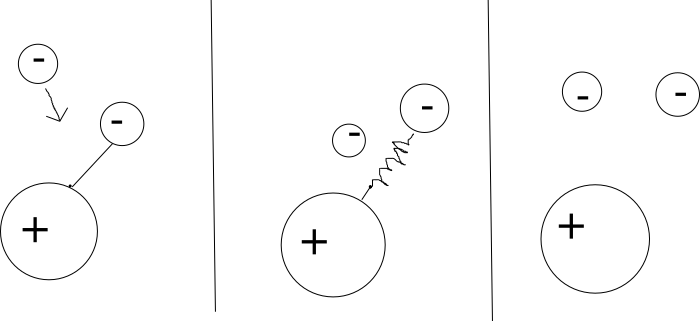
\includegraphics[width=0.95\linewidth]{Figures/hydrogensketchion.png} 
\end{column}
\end{columns}
\end{frame}

\begin{frame}{Ionisation, recombination and ionisation potential in two-fluid shocks}
\footnotesize
\begin{gather}
\frac{\partial \rho _{\text{n}}}{\partial t} + \nabla \cdot (\rho _{\text{n}} \textbf{v}_{\text{n}})= \Gamma _{rec} \rho _{\rm p} - \Gamma _{ion} \rho _{\rm n}, \label{eqn:neutral1}\tag{5} \\
\frac{\partial}{\partial t}(\rho _{\text{n}} \textbf{v}_{\text{n}}) + \nabla \cdot (\rho _{\text{n}} \textbf{v}_{\text{n}} \textbf{v}_{\text{n}} + P_{\text{n}} \textbf{I}) = -\alpha _c \rho_{\text{n}} \rho_{\text{p}} (\textbf{v}_{\text{n}}-\textbf{v}_{\text{p}}) + \Gamma _{rec} \rho _{\rm p} \textbf{v}_{\rm p} - \Gamma _{ion} \rho_{\rm n} \textbf{v}_{\rm n},\tag{6} \\
\frac{\partial e_{\text{n}}}{\partial t} + \nabla \cdot \left[\textbf{v}_{\text{n}} (e_{\text{n}} +P_{\text{n}}) \right] = -\alpha _c \rho _{\text{n}} \rho _{\text{p}} \left[ \frac{1}{2} (\textbf{v}_{\text{n}} ^2 - \textbf{v}_{\text{p}} ^2)+ \frac{3}{2} \left(\frac{P_{\rm n}}{\rho_{\rm n}}-\frac{1}{2}\frac{P_{\rm p}}{\rho_{\rm p}}\right) \right] \nonumber \\ \hspace{0.5cm}+ \frac{1}{2} \left( \Gamma _{rec} \rho _{\rm p} \textbf{v}_{\rm p} ^2 - \Gamma _{ion} \rho _{\rm n} \textbf{v}_{\rm n} ^2 \right) +\frac{1}{ (\gamma-1)} \left( \frac{1}{2} \Gamma _{rec} P_{\rm p} -\Gamma _{ion} P_{\rm n} \right), \tag{7}\\
%e_{\text{n}} = \frac{P_{\text{n}}}{\gamma -1} + \frac{1}{2} \rho _{\text{n}} v_{\text{n}} ^2, \label{eqn:neutral2} \\
\frac{\partial \rho _{\text{p}}}{\partial t} + \nabla \cdot (\rho_{\text{p}} \textbf{v}_{\text{p}}) = - \Gamma _{rec} \rho _{\rm p} + \Gamma _{ion} \rho _{\rm n} \label{eqn:plasma1}\tag{8}\\
\frac{\partial}{\partial t} (\rho_{\text{p}} \textbf{v}_{\text{p}})+ \nabla \cdot \left( \rho_{\text{p}} \textbf{v}_{\text{p}} \textbf{v}_{\text{p}} + P_{\text{p}} \textbf{I} - \textbf{B B} + \frac{\textbf{B}^2}{2} \textbf{I} \right) = \alpha _c \rho_{\text{n}} \rho_{\text{p}}(\textbf{v}_{\text{n}} - \textbf{v}_{\text{p}}) - \Gamma _{rec} \rho _{\rm p} \textbf{v}_{\rm p} + \Gamma _{ion} \rho_{\rm n} \textbf{v}_{\rm n},\tag{9}\\
\frac{\partial}{\partial t} \left( e_{\text{p}} + \frac{\textbf{B}^2}{2} \right) + \nabla \cdot \left[ \textbf{v}_{\text{p}} ( e_{\text{p}} + P_{\text{p}}) -  (\textbf{v}_{\rm p} \times \textbf{B}) \times \textbf{B} \right]  =  \alpha _c \rho _{\text{n}} \rho _{\text{p}} \left[ \frac{1}{2} (\textbf{v}_{\text{n}} ^2 - \textbf{v}_{\text{p}} ^2)+ \frac{3}{2} \left(\frac{P_{\rm n}}{\rho_{\rm n}}-\frac{1}{2}\frac{P_{\rm p}}{\rho_{\rm p}}\right) \right] \nonumber \\ \hspace{0.5cm}- \frac{1}{2} \left( \Gamma _{rec} \rho _{\rm p} \textbf{v}_{\rm p} ^2 - \Gamma _{ion} \rho _{\rm n} \textbf{v}_{\rm n} ^2 \right) \mathcolorbox{yellow}{- \phi_I + A_{heat}} -\frac{1}{ (\gamma-1)} \left( \frac{1}{2} \Gamma _{rec} P_{\rm p} -\Gamma _{ion} P_{\rm n} \right), \label{eqn:ep} \tag{10}\\
\frac{\partial \textbf{B}}{\partial t} - \nabla \times (\textbf{v}_{\text{p}} \times \textbf{B}) = 0.\tag{11}
%e_{\text{p}} = \frac{P_{\text{p}}}{\gamma -1} + \frac{1}{2} \rho _{\text{p}} v_{\text{p}} ^2, \\
%\nabla \cdot \textbf{B} = 0,\label{eqn:plasma2}
\end{gather}
\end{frame}

\begin{frame}{Collisional ionisation/recombination}
\begin{columns}
\begin{column}{0.4\textwidth}
\begin{enumerate}
\item Collisional ionisation only.
\item Shocks are highly dynamic and can have large temperature jumps.
\item Need to account for ionisation and recombination.
\item Kinetic energy of a free electron used to release a bound electron during ionisation.
\end{enumerate}
\end{column}
\begin{column}{0.6\textwidth}
Empirical rates for hydrogen from Voranov (1997) and Smirnov (2003) in normalised form:
    \begin{gather}
    \Gamma_{rec} = \frac{\rho_{\rm p}}{\sqrt{T_{\rm p}}} \frac{\sqrt{T_f}}{\xi _{{\rm p}0}} \tau _{IR} = F(T) \rho_{\rm p}, \\
    \Gamma_{ion} = \rho_{\rm p} \frac{\mbox{e} ^{-\chi} \chi ^{0.39} }{0.232 + \chi} \frac{\hat{R}}{\xi _{{\rm p}0}} \tau _{IR} = G(T) \rho_{\rm p}, \\
    \chi = 13.6 \frac{T_f}{T_{e0} T_{\rm p}}, \\
    \hat{R} = \frac{2.91 \times 10 ^{-14}}{2.6 \times 10^{-19}} \sqrt{T_{e0}},
    %\\ T_f = \frac{1}{4} \beta \gamma \frac{2 \xi_{p0}}{\xi_{n0} +2 \xi_{p0}}
\end{gather}
\end{column}
\end{columns}
\end{frame}

\begin{frame}{Ionisation, recombination and ionisation potential}
\begin{columns}
\begin{column}{0.4\textwidth}
\begin{itemize}
    \item Ionisation potential term: macroscopic energy lost during ionisation. %Requires a heating term to balance.
    \item We perform 1D two-fluid simulations of ionisation, recombination and ionisation potential terms in a slow-mode shock.
\end{itemize}
\begin{gather}
    \phi _I = \Gamma _{ion} \rho _{\rm n} \hat{\phi}. \nonumber \\
    A_{heat}=\phi _I(t=0)=constant \nonumber
\end{gather}
\end{column}
\begin{column}{0.6\textwidth}
\footnotesize
\begin{itemize}
    \item On recombination only the proton thermal energy is transferred to the neutral fluid. The thermal energy previously held by the recombined electron remains in the electron fluid (and with that the plasma as a whole) as it is transferred to the free electron involved in the three-body recombination.
    \item The electron is assumed to recombine to an arbitrary level of the atom. 
    \item We assume all the other energy involved in the recombination process (coming from the work done on the recombining electron by the proton electric field) is released as a photon.
    \item The medium is assumed to be optically thin.
    \item The electron in any neutral cascades down from higher levels to the ground state by releasing photons.
    \item To ionise the neutral from the ground state through collisions with another electron, work has to be done by the free electron to release the bound electron, resulting in an energy loss. As we assume this happens to electrons in the ground state, the work done is 13.6eV.
\end{itemize}
\end{column}
\end{columns}
\end{frame}


% \begin{frame}{Ionisation, recombination and ionisation potential in two-fluid shocks}
% \begin{gather}
%     \frac{\partial \rho _{\text{n}}}{\partial t} + \nabla \cdot (\rho _{\text{n}} \textbf{v}_{\text{n}})= \Gamma _{rec} \rho _{\rm p} - \Gamma _{ion} \rho _{\rm n}
% \end{gather}
% When ionisation and recombination are studied (with ionisation potential neglected), the ionisation equilibrium can be easily determined from the continuity equation as:
% \begin{gather}
%     \Gamma _{ion} \rho _{\rm n} = \Gamma _{rec} \rho_{\rm p}, \\
%     \Gamma _{ion}/\Gamma _{rec} = \rho _{\rm p}/ \rho _{\rm n}.
% \end{gather}
% Therefore, the only constraint for ionisation equilibrium is that the ratio of ionisation/recombination rates equals the ratio of plasma/neutral densities. 
% \end{frame}

% \begin{frame}{Equilibrium conditions - IR model}
% \begin{columns}
% \begin{column}{0.55\textwidth}
% \begin{itemize}
%     \item Ionisation and recombination (but without ionisation potential) equilibrium conditions
%     \item The only constraint for ionisation equilibrium is that the ratio of ionisation to recombination rates equals the ratio of plasma to neutral densities. 
%     \item For a given temperature, equilibrium exists at a certain neutral fraction.
%     \item As such, ionisation equilibrium relies on the ratio of densities, and not the specific density values.
% \end{itemize}
% \end{column}
% \begin{column}{0.45\textwidth}
% \begin{gather}
%     \frac{\partial \rho _{\text{n}}}{\partial t} + \nabla \cdot (\rho _{\text{n}} \textbf{v}_{\text{n}})= \Gamma _{rec} \rho _{\rm p} - \Gamma _{ion} \rho _{\rm n} \\
%     \Gamma _{rec} \rho _p = \Gamma _{ion} \rho _n \\
%     \frac{\Gamma_{rec}}{\Gamma_{ion}} = \frac{\rho _n}{\rho_p}
% \end{gather}
% \end{column}
% \end{columns}
% \end{frame}

\begin{frame}{Equilibrium conditions - IRIP model}
\textbf{Ionisation, recombination and ionisation potential equilibrium conditions}
\begin{columns}
\begin{column}{0.45\textwidth}
\begin{figure}
    \centering
    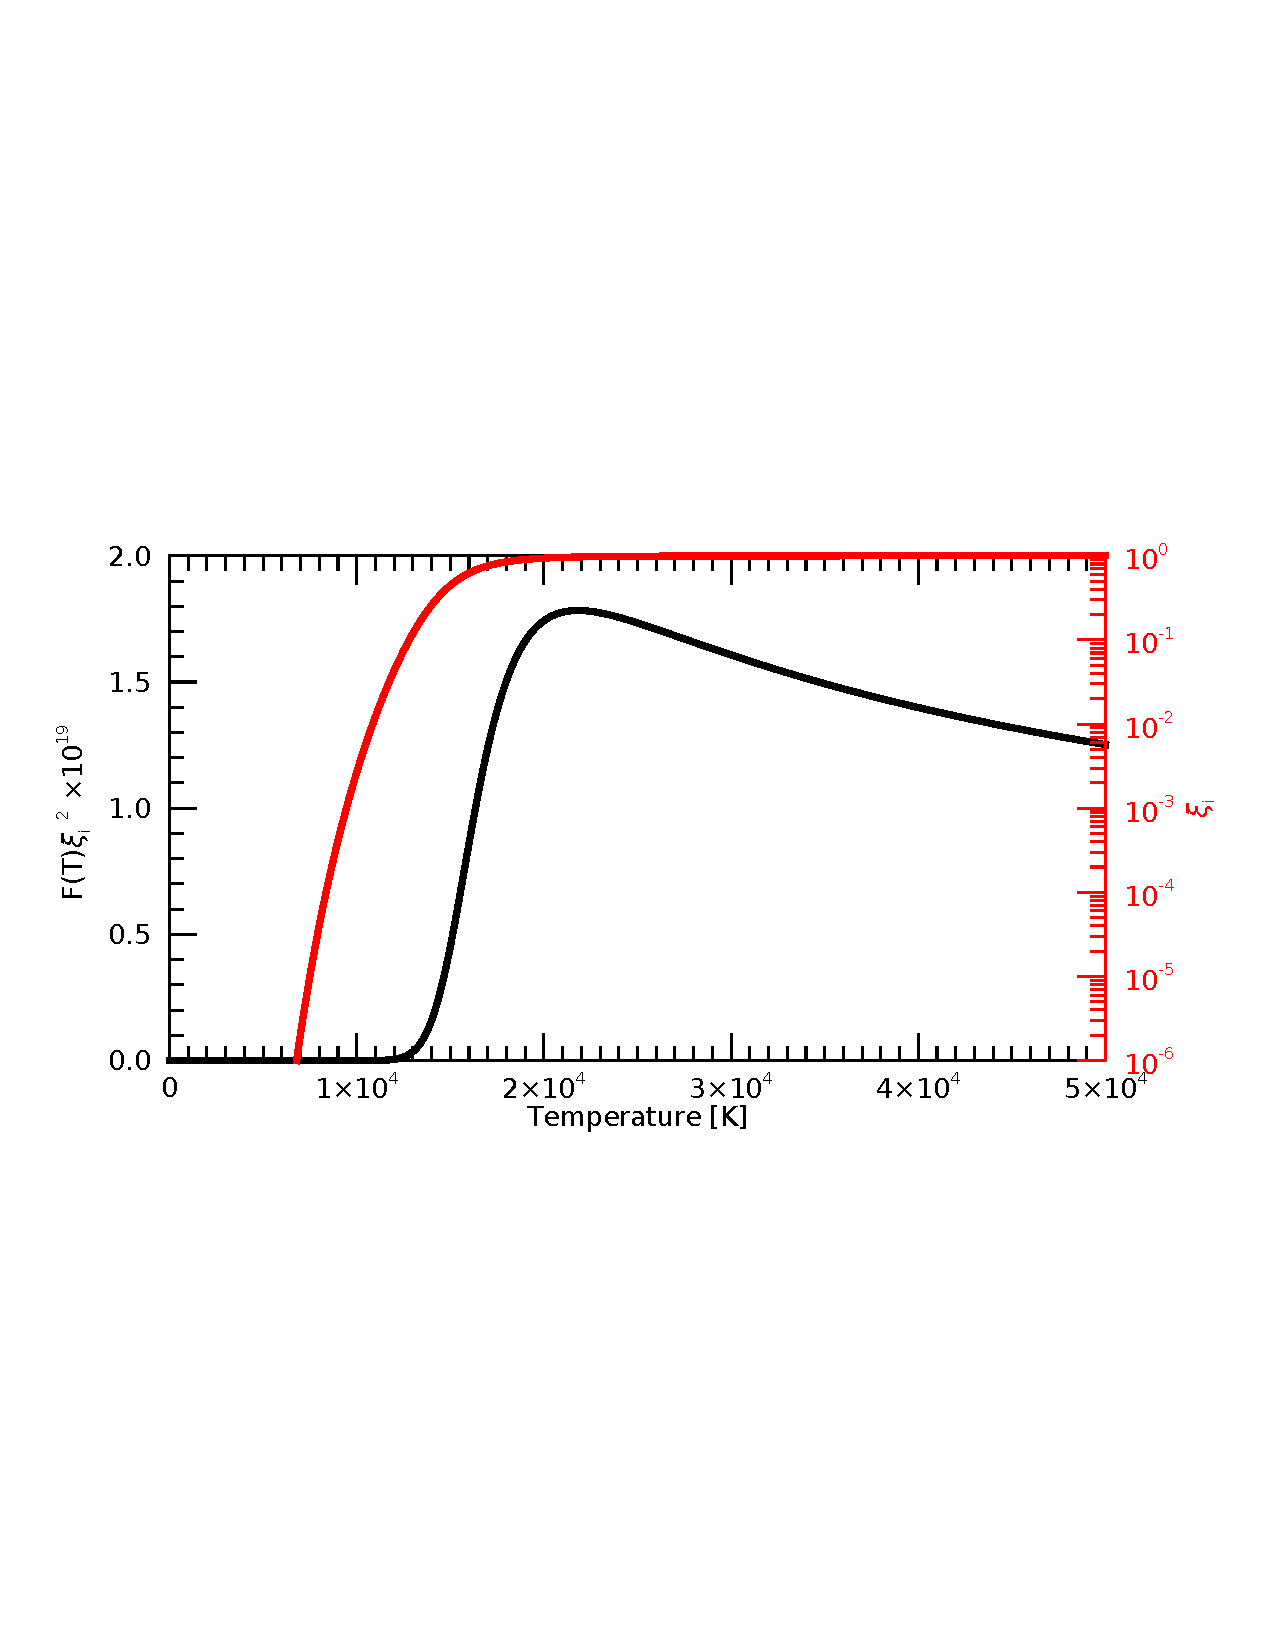
\includegraphics[width=0.95\linewidth,clip=true,trim=0.9cm 8.8cm 0.9cm 8.8cm]{eqltest3.pdf}
    \caption{$F(T) \xi_i^2$ as a function of temperature in dimensional form. Red line shows the ionisation fraction $\xi_i$ for the associated temperature.}
    \label{fig:eqltest}
\end{figure}
\end{column}
\begin{column}{0.55\textwidth}
Including the ionisation potential for an equilibrium, we require that the ionisation potential and heating terms balance:
\begin{gather}
    \hat{\phi} \Gamma _{ion} \rho_{\rm n} = \hat{\phi} \Gamma _{ion} (t=0) \rho _{\rm n} (t=0), \\
    \Gamma _{ion} \rho_{\rm n} = \Gamma _{rec} \rho_{\rm p} = \Gamma _{ion} (t=0) \rho _{\rm n} (t=0) =\mbox{const.} \\
    G(T)\rho_{\rm p} \rho_{\rm n} = F(T) \rho_{\rm p} ^2 = \mbox{const.} \\
    F(T) \xi_i ^2 \rho ^2 = \mbox{const.} \\
     \xi_i=\frac{1}{\frac{F(T)}{G(T)} +1}.
\end{gather}
\textbf{A compressible partially-ionised shock must cool across the interface!}
\end{column}
\end{columns}
\end{frame}

% \begin{frame}{IR shock jumps}
% \textbf{Ionisation and recombination (without ionisation potential)}
% \small
% \begin{gather}
% \nabla \cdot (\rho _{\text{n}} \textbf{v}_{\text{n}})= S_{mass}, \\
% \nabla \cdot (\rho _{\text{n}} \textbf{v}_{\text{n}} \textbf{v}_{\text{n}} + P_{\text{n}} \textbf{I}) = S_{mom}, \\
% \nabla \cdot \left[\textbf{v}_{\text{n}} (e_{\text{n}} +P_{\text{n}}) \right] = S_{eng}, \\
% \nabla \cdot (\rho_{\text{p}} \textbf{v}_{\text{p}}) = - S_{mass},\\
% \nabla \cdot \left( \rho_{\text{p}} \textbf{v}_{\text{p}} \textbf{v}_{\text{p}} + P_{\text{p}} \textbf{I} - \textbf{B B} + \frac{\textbf{B}^2}{2} \textbf{I} \right) = - S_{mom}, \\
% \nabla \cdot \left[ \textbf{v}_{\text{p}} ( e_{\text{p}} + P_{\text{p}}) -  (\textbf{v}_p \times \textbf{B}) \times \textbf{B} \right] =  -S_{eng}, \\
% \nabla \times (\textbf{v}_{\text{p}} \times \textbf{B}) = 0, \\
% S_{mass}=\Gamma _{rec} \rho _p - \Gamma _{ion} \rho _n, \label{eqn:smass}\\
% S_{mom}=-\alpha _c \rho_{\text{n}} \rho_{\text{p}} (\textbf{v}_{\text{n}}-\textbf{v}_{\text{p}}) + \Gamma _{rec} \rho _p \textbf{v}_{p} - \Gamma _{ion} \rho_n \textbf{v}_n, \label{eqn:smom}\\
% S_{eng} =-\alpha _c \rho _{\text{n}} \rho _{\text{p}} \left[ \frac{1}{2} (\textbf{v}_{\text{n}} ^2 - \textbf{v}_{\text{p}} ^2)+ \frac{3}{2} \left(\frac{P_n}{\rho_n}-\frac{1}{2}\frac{P_p}{\rho_p}\right) \right] \nonumber \\ \hspace{1.0cm}+ \frac{1}{2} \left( \Gamma _{rec} \rho _p \textbf{v}_p ^2 - \Gamma _{ion} \rho _n \textbf{v}_n ^2 \right) +\frac{1}{ (\gamma-1)} \left( \frac{1}{2} \Gamma _{rec} P_p -\Gamma _{ion} P_n \right). \label{eqn:seng} 
% \end{gather}
% \end{frame}

% \begin{frame}{IR shock jumps}
% \textbf{Ionisation and recombination (without ionisation potential)}
% \begin{gather}
%     \left[\xi_n \rho_{B} v_{nx} +(1-\xi_n) \rho_{B} v_{px}  \right]^u _d = 0,  \\
%     \left[\rho_{B} v_{nx}^2 + \frac{\xi _n}{ 2-\xi_n} P_{B} +(1-\xi_n)\rho _{B} v_{px}^2 \right. \nonumber \\ \hspace{0.5cm} \left. +\frac{2(1-\xi _n)}{2-\xi_n} P_{B} +\frac{B_y^2}{2} \right]^u _d = 0, \\
%     \left[\xi_n \rho_{B} v_{nx} v_{ny}  + (1-\xi_n) \rho _{B} v_{px} v_{py} -B_x B_y \right]^u _d = 0, \\
%     \left[ v_{nx} \left( \frac{\gamma}{\gamma -1} \frac{\xi _n}{ 2-\xi_n} P_B + \frac{1}{2} \xi _n \rho _B v_n^2 \right) \right. \nonumber \\ \hspace{0.5cm} \left. +v_{px} \left( \frac{\gamma}{\gamma -1} \frac{2(1-\xi _n)}{ 2-\xi_n} P_B + \frac{1}{2} (1-\xi _n) \rho _B v_p^2 \right) \right]^u _d =0, \\
%     \left[B_x \right]^u _d = 0,\\
%     \left[v_{px} B_{y} -v_{py} B_x   \right]^u _d = 0,
% \end{gather}
% \end{frame}

% \begin{frame}{IR shock jumps}
% \textbf{Ionisation and recombination (without ionisation potential)}
% \begin{columns}
% \begin{column}{0.45\textwidth}
% \begin{gather}
%     \left[\rho_B v_x  \right]^u _d = 0,  \\
%     \left[\rho_B v_x^2 +P_B +\frac{B_y^2}{2} \right]^u _d = 0, \\
%     \left[\rho_B v_x v_y -B_x B_y \right]^u _d = 0, \\
%     \left[ v_{x} \left( \frac{\gamma}{\gamma -1} P_B + \frac{1}{2} \rho _B v^2 \right) \right]^u _d =0,\\
%     \left[B_x \right]^u _d = 0, \\
%     \left[v_x B_y -v_y B_x   \right]^u _d = 0. 
% \end{gather}
% \end{column}
% \begin{column}{0.55\textwidth}
% \footnotesize
% \begin{itemize}
%     \item Collisional ionisation and recombination (without ionisation potential) has the same solution as MHD:
% \end{itemize}
% \begin{gather}
%     A_x ^{\text{u}2} = \left[ A_x ^{\text{d}2} \left( \frac{\gamma-1}{\gamma} \left( \frac{\gamma+1}{\gamma -1} -\tan ^2 \theta \right) \left(A_x ^{\text{d}2} -1 \right) ^2 \right. \right. \nonumber\\ 
%     + \left. \left. \tan ^2 \theta \left( \frac{\gamma-1}{\gamma} A_x ^{\text{d}2} -1 \right) \left(A_x ^{\text{d}2} -2 \right) \right) - \frac{\beta}{ \cos ^2 \theta } \left( A_x ^{\text{d}2} -1 \right) ^2 \right]  \nonumber\\
%     / \left[ \frac{\gamma -1}{\gamma} \frac{\left( A_x ^{\text{d}2}-1 \right) ^2}{ \cos ^2 \theta } - A_ x ^{\text{d}2} \tan ^2 \theta \left( \frac{\gamma -1}{\gamma} A_x ^{\text{d}2} -1 \right) \right].
% \end{gather}
% \end{column}
% \end{columns}
% \end{frame}

\begin{frame}{IRIP shock jumps}
\textbf{Ionisation recombination and ionisation potential}
\begin{gather}
\nabla \cdot (\rho _{\text{n}} \textbf{v}_{\text{p}})= S_{mass}, \\
\nabla \cdot (\rho _{\text{n}} \textbf{v}_{\text{n}} \textbf{v}_{\text{n}} + P_{\text{n}} \textbf{I}) = S_{mom}, \\
\nabla \cdot \left[\textbf{v}_{\text{n}} (e_{\text{n}} +P_{\text{n}}) \right] = S_{eng}, \\
\nabla \cdot (\rho_{\text{p}} \textbf{v}_{\text{p}}) = - S_{mass},\\
\nabla \cdot \left( \rho_{\text{p}} \textbf{v}_{\text{p}} \textbf{v}_{\text{p}} + P_{\text{p}} \textbf{I} - \textbf{B B} + \frac{\textbf{B}^2}{2} \textbf{I} \right) = - S_{mom}, \\
\nabla \cdot \left[ \textbf{v}_{\text{p}} ( e_{\text{p}} + P_{\text{p}}) -  (\textbf{v}_p \times \textbf{B}) \times \textbf{B} \right] =  -S_{eng} -\phi _I +A_{heat}, \\
\nabla \times \left(\textbf{v}_{\text{p}} \times \textbf{B} \right) = 0
\end{gather}
\end{frame}

\begin{frame}{IRIP shock jumps}
\textbf{Ionisation recombination and ionisation potential}
\begin{gather}
    \nabla \cdot (\rho _n \textbf{v}_n +\rho _p \textbf{v}_n)= 0, \\
    \nabla \cdot (\rho _n \textbf{v}_n \textbf{v}_n + P_n \textbf{I} +\rho _p \textbf{v}_p \textbf{v}_p + P_p \textbf{I}) = 0, \\
    \nabla \cdot \left[\textbf{v}_n (e_n +P_n) +\textbf{v}_p (e_p +P_p) -  (\textbf{v}_p \times \textbf{B}) \times \textbf{B} \right] = -\phi_I + A_{heat}, \label{eqn:iripen} \\
    \nabla \times \left(\textbf{v}_p \times \textbf{B} \right) = 0, \\
    \nabla \cdot \textbf{B} = 0.
\end{gather}
\end{frame}

\begin{frame}{Shock jumps}
\begin{columns}
\begin{column}{0.45\textwidth}
\begin{gather}
    \left[\rho_B v_x  \right]^u _d = 0, \label{eqn:iripjump1} \\
    \left[\rho_B v_x^2 +P_B +\frac{B_y^2}{2} \right]^u _d = 0, \\
    \left[\rho_B v_x v_y -B_x B_y \right]^u _d = 0, \\
    \left[B_x \right]^u _d = 0, \\
    \left[v_x B_y -v_y B_x   \right]^u _d = 0, \label{eqn:iripjump2} \\
    \left[ F(T) \xi_i^2 \rho_B^2 \right]^u _d=0.
\end{gather}
\end{column}
\begin{column}{0.55\textwidth}
\begin{gather}
    \frac{T^d}{T^u} = \frac{A_x^{d2}}{A_x^{u2}} \left[1 + \frac{2}{\beta (1+ \tan ^2 (\theta))} \times \nonumber \right. \\ \left. \hspace{0.7cm} \left[ A_x^{u2}-A_x^{d2} + \frac{\tan ^2 (\theta)}{2} \left(1 - \left(\frac{A_x^{u2}-1}{A_x^{d2}-1}\right)^2\right)  \right] \right], \label{eqn:irtjump} \\
%    \frac{F(T ^d)}{F(T^u)} \left( \frac{F(T^u)/G(T^u) +1}{F(T^d)/G(T^d) +1} \right)^2= \frac{1}{r^2}. \label{eqn:ftjump}
    \frac{F(T ^d)}{F(T^u)} \left( \frac{F(T^u)/G(T^u) +1}{F(T^d)/G(T^d) +1} \right)^2= \frac{A_x^{d4}}{A_x^{u4}}. \label{eqn:ftjump}
\end{gather}
\end{column}
\end{columns}
\end{frame}

\begin{frame}{Shock jumps}
\begin{figure}
    \centering
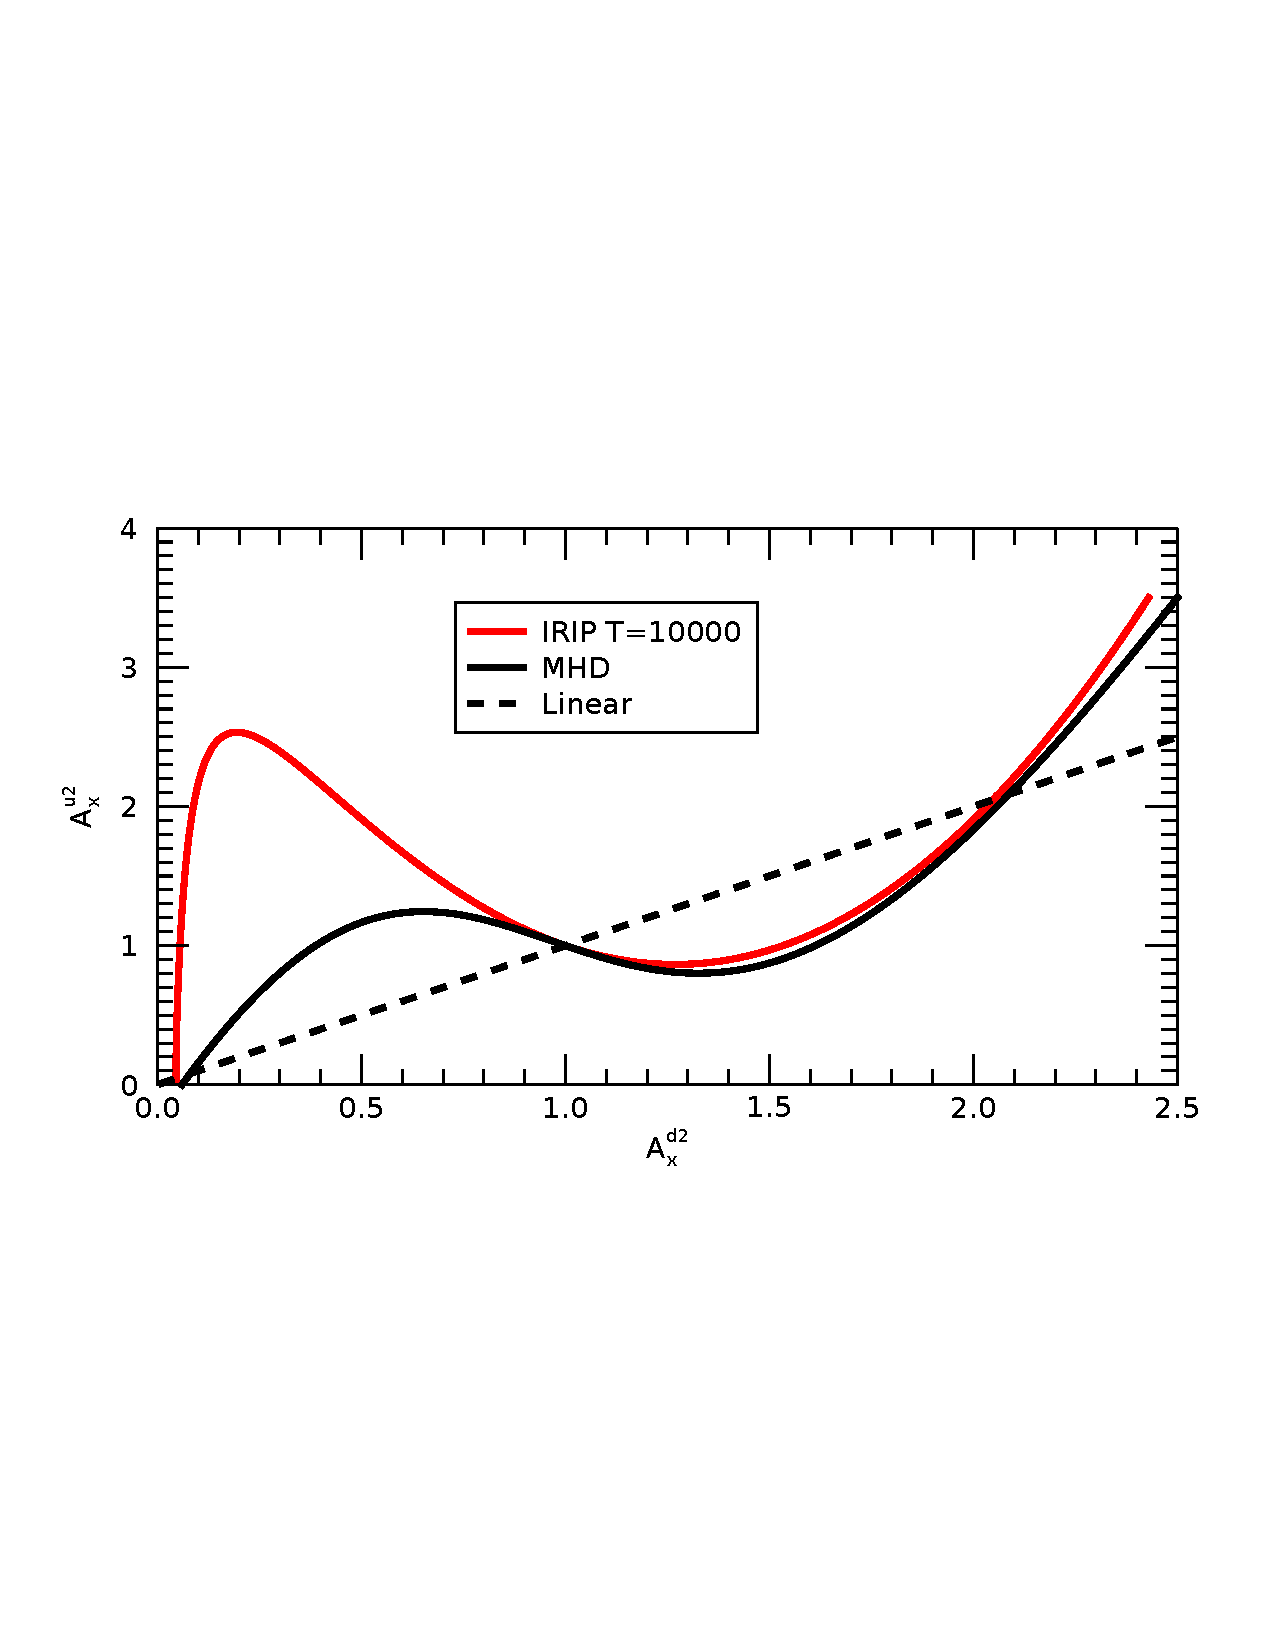
\includegraphics[width=0.7\linewidth,clip=true,trim=1.0cm 8.2cm 1.2cm 8.3cm]{tjumpplotex.pdf}
    \caption{Solutions to the shock jump equations for the IRIP (red) and MHD (black) equations relating the upstream ($^u$) and downstream ($^d$) Alfv\'en Mach numbers $A_x$. The trivial solution ($A_x^{d}=A_x^{u}$) exists for both sets of equations. The parameters used for this plot are $T_0 = 10000$ K, $\beta = 0.1$, $\theta =\pi/4$ and $\gamma =5/3$.}
    \label{fig:tjumpex}
\end{figure}
\end{frame}

\begin{frame}{Numerical model}
\begin{columns}
\begin{column}{0.4\textwidth}
\begin{enumerate}
\item 1D shocks in two-fluid partially-ionised plasma using (P\underline{I}P) code.
\item Investigate shock substructure.
\item Initial conditions produce slow-mode shock.
\item Mimics shocks produced by Petschek-type reconnection.
\item Equilibrium recombination timescale set to $10^{-3}$ of collisional timestep.
\item 256000 grid cells, 1st order HLLD solver, explicit integration of source terms.
\end{enumerate}
\end{column}
\begin{column}{0.6\textwidth}
\begin{eqnarray}
B_x &=& 0.1 \\
B_y &=& -1.0 (x>0), 1.0 (x<0) \\
\rho _n &=& \xi _n \rho _{tot} \\
\rho _p &=& \xi _i \rho _{tot} = (1- \xi _n) \rho _{tot} \\
P_n &=& \frac{\xi _n}{\xi_n + 2 \xi _i} P_{tot} =  \frac{\xi _n}{\xi_n + 2 \xi _i} \beta \frac{B_0 ^2}{2} \\
P_p &=& \frac{2 \xi _i}{\xi_n + 2 \xi _i} P_{tot} =  \frac{2 \xi _i}{\xi_n + 2 \xi _i} \beta \frac{B_0 ^2}{2}
\end{eqnarray}
\end{column}
\end{columns}
\end{frame}

\begin{frame}{Numerical simulation - shock properties}
\begin{figure}
    \centering
\includegraphics[width=0.85\linewidth,clip=true,trim=1.5cm 7.8cm 1.5cm 7.8cm]{radfull4.pdf}
%\includegraphics[width=0.95\linewidth,clip=true,trim=0.2cm 0.1cm 1.5cm 0.1cm]{figures/radfull2.png}
    \caption{Context figure for the equilibrium state in the MHD (black), IRIP (solid) and IR (dashed) cases. The blue (red) line is for the plasma (neutral) species for the two-fluid cases.}
    \label{fig:radfull}
\end{figure}
\end{frame}

\begin{frame}{Numerical simulation - energies}
\begin{figure}
    \centering
%\includegraphics[width=0.85\linewidth,clip=true,trim=0.9cm 7.8cm 1.5cm 7.8cm]{rareeng2.pdf}
\includegraphics[width=0.85\linewidth,clip=true,trim=10.9cm 7.8cm 1.5cm 7.8cm]{rareeng2.pdf}
    \caption{Energies across the system for the MHD (black) and IRIP cases (red neutrals, blue plasma). The quantity $A_{heat}- \phi _I$ shows the balance between the heating and loss terms in the energy equation where red denotes net energy addition (heating) and blue is net energy loss (cooling).}
    \label{fig:rareeng}
\end{figure}
\end{frame}

\begin{frame}{Numerical simulation - slow-mode shock}
\begin{figure}
    \centering
\includegraphics[width=0.85\linewidth,clip=true,trim=0.9cm 7.8cm 1.5cm 7.8cm]{radslow2.pdf}
    \caption{Close-up of the slow mode shock for the IRIP model showing $v_x$ velocity (top left), temperature (top right) and density (lower left) for plasma (blue) and neutral (red) species. The lower right panel shows the ionisation (orange) and recombination (green) rates.}
    \label{fig:radslow}
\end{figure}
\end{frame}

% \begin{frame}{Shock jumps}
% \begin{figure}
%     \centering
% \includegraphics[width=0.7\linewidth,clip=true,trim=0.9cm 7.8cm 1.5cm 7.8cm]{sframe.pdf}
%     \caption{Alfven Mach numbers for the MHD (black) and plasma (blue) based on the bulk density. The red line shows the neutral sonic Mach number.}
%     \label{fig:mach}
% \end{figure}
% \end{frame}

% \begin{frame}{Time evolution}
% \begin{figure}
%     \centering
% \includegraphics[width=0.8\linewidth,clip=true,trim=0.9cm 7.8cm 0.5cm 7.8cm]{timeseries3.pdf}
%     \caption{Time series for the IRIP case after 1 (top), 10 (middle) and 100 (lower) collisional times showing the $v_x$ velocity (left), temperature (centre), and ionisation and recombination rates (right).}
%     \label{fig:timeseries}
% \end{figure}
% \end{frame}

% \begin{frame}{Different recombination timescales}
% \begin{columns}
% \begin{column}{0.5\textwidth}
% \vspace{-1cm}
% \begin{figure}
%     \centering
% \includegraphics[width=0.95\linewidth,clip=true,trim=0.95cm 8.3cm 10.5cm 7.8cm]{widthradt2_vx.pdf}
% %    \caption{Plasma (blue) and neutral (red) $v_x$ velocities for recombination timescales of $10^{-3}$, $10^{-5}$, $10^{-6}$, $10^{-7}$, from top to bottom.}
%     \label{fig:shockwidthvx}
% \end{figure}
% \end{column}
% \begin{column}{0.42\textwidth}
% \begin{figure}
%     \centering
% \includegraphics[width=0.95\linewidth,clip=true,trim=0.9cm 7.8cm 1.5cm 7.8cm]{radttemp.pdf}
% %    \caption{Plasma (solid) and neutral (dashed) temperatures for different initial recombination rates. The orange dashed line shows the downstream MHD temperature.}
%     \label{fig:radt}
% \end{figure}
% \begin{figure}
%     \centering
% \includegraphics[width=0.95\linewidth,clip=true,trim=0.7cm 7.8cm 1.5cm 7.8cm]{widthradt2_xi.pdf}
%     \caption{Ionisation fraction across the shock for different recombination rates.}
%     \label{fig:shockwidthxi}
% \end{figure}
% \end{column}
% \end{columns}
% \end{frame}

\begin{frame}{Cooling through the shock}
\begin{columns}
\begin{column}{0.5\textwidth}
\begin{figure}
    \centering
%\includegraphics[width=0.95\linewidth,clip=true,trim=0.9cm 7.8cm 1.5cm 7.8cm]{figures/widthradt2_sw.pdf}
%    \caption{Finite width of the shock as a function of upstream recombination rates.}
    \includegraphics[width=0.95\linewidth,clip=true,trim=0.9cm 7.8cm 1.2cm 7.8cm]{shockloss.pdf}
    \caption{Finite width of the shock (black line) as a function of the initial recombination rates. Integrated cooling for a parcel of fluid travelling through the shock is shown by the red line.}
    \label{fig:shockwidthsw}
\end{figure}
\end{column}
\begin{column}{0.42\textwidth}
\begin{itemize}
    \item Calculate the cooling experienced by a particle as it passes through the shock for different reference recombinaton timescales.
    \item Particle cools because $\phi _{I} > A_{heat}$.
    \item Molecules that should be disassociated survive interstellar medium shocks. Radiative losses decrease maximum obtained temperature and hence they survive (Drain+1993).
    \item Possible increase in line broadening here.
    \item Needs further study!
\end{itemize}
\end{column}
\end{columns}
\end{frame}

% \begin{frame}{Application to reconnection}
%     \centering
% \includegraphics[width=0.95\linewidth,clip=true,trim=0.1cm 0.1cm 0.1cm 0.1cm]{plasmoid_timeevo.png}
% %    \caption{Finite width of the shock as a function of upstream recombination rates.}
% %    \includegraphics[width=0.95\linewidth,clip=true,trim=0.9cm 7.8cm 1.2cm 7.8cm]{shockloss.pdf}
% %    \caption{Finite width of the shock (black line) as a function of the initial recombination rates. Integrated cooling for a parcel of fluid travelling through the shock is shown by the red line.}
% %    \label{fig:shockwidthsw}
% \end{frame}

% \begin{frame}{Application to reconnection}
% \begin{columns}
% \begin{column}{0.5\textwidth}
% \begin{figure}
%     \centering
% \includegraphics[width=0.95\linewidth]{plasmoid_recrate.png}
% %    \caption{Finite width of the shock as a function of upstream recombination rates.}
% %    \includegraphics[width=0.95\linewidth,clip=true,trim=0.9cm 7.8cm 1.2cm 7.8cm]{shockloss.pdf}
% %    \caption{Finite width of the shock (black line) as a function of the initial recombination rates. Integrated cooling for a parcel of fluid travelling through the shock is shown by the red line.}
% %    \label{fig:shockwidthsw}
% \end{figure}
% \end{column}
% \begin{column}{0.42\textwidth}
% \begin{itemize}
%     \item Ionisation/recombination lowers reconnection rate
%     \item Temperature increase in reconnection region (Ohmic diffusion, adiabatic) leads to ionisation
%     \item Larger plasma density lowers Lundquist number 
%     \item prevents secondary plasmoids forming
% \end{itemize}
% \end{column}
% \end{columns}
% \end{frame}

% \begin{frame}{Application to reconnection}
% \begin{columns}
% \begin{column}{0.49\textwidth}
% \begin{figure}
%     \centering
% \includegraphics[width=0.95\linewidth]{plasmoid_temp.png}
% \end{figure}
% \end{column}
% \begin{column}{0.49\textwidth}
% \begin{figure}
%     \centering
% \includegraphics[width=0.95\linewidth]{plasmoid_cooling.png}
% \end{figure}
% \end{column}
% \end{columns}
% \end{frame}

\begin{frame}{Conclusions}
\begin{itemize}
    \item \textbf{Do partially ionised shocks always heat the solar chromosphere - no.}
    \item Ionisation potential fundamentally changes the behaviour of shocks.
    \item Equilibrium can only exist at certain densities (as opposed to neutral fractions when only ionisation/recombination is considered).
    \item A partially-ionised compressible shock must cool across the interface.
    \item IRIP shocks can be overcompressed (far beyond the MHD limit of $r=4$)
    \item Ionisation/recombination rates are significantly enhanced in the shock.
    \item Snow \& Hillier, 2021, A\&A, 645, A81 (also on arXiv)
\end{itemize}
\end{frame}

% \begin{frame}{Problems?}
% \begin{itemize}
%     \item Empirical rates fitted to temperatures above 1eV (11600 K).
%     \item Interested in media cooler than this.
%     \item Assumed ground state only - hydrogen exists in multiple excited states.
%     \item Collisional ionisation only - radiative can be important.
% \end{itemize}
% \end{frame}

% \begin{frame}{Future work}
% \includegraphics[width=0.9\linewidth]{simlevels_rad_thick_10000.png}
% \end{frame}

% \begin{frame}{Ionisation/recombination rates in normalised form}
% Empirical rates from Smirnov (2003) and Voranov (1997) in normalised form:
%     \begin{gather}
%     \Gamma_{rec} = \frac{\rho_{\rm p}}{\sqrt{T_{\rm p}}} \frac{\sqrt{T_f}}{\xi _{{\rm p}0}} \tau _{IR} = F(T) \rho_{\rm p}, \\
%     \Gamma_{ion} = \rho_{\rm p} \frac{\mbox{e} ^{-\chi} \chi ^{0.39} }{0.232 + \chi} \frac{\hat{R}}{\xi _{{\rm p}0}} \tau _{IR} = G(T) \rho_{\rm p}, \\
%     \chi = 13.6 \frac{T_f}{T_{e0} T_{\rm p}}, \\
%     \hat{R} = \frac{2.91 \times 10 ^{-14}}{2.6 \times 10^{-19}} \sqrt{T_{e0}},
%     %\\ T_f = \frac{1}{4} \beta \gamma \frac{2 \xi_{p0}}{\xi_{n0} +2 \xi_{p0}}
% \end{gather}
% \end{frame}



% \begin{frame}{Corrugation instability}
% \begin{columns}
% \begin{column}{0.5\textwidth}
%     \includegraphics[width=0.95\linewidth,clip=true,trim=1.1cm 7.8cm 1.5cm 7.8cm]{icstab.pdf} \\
%      A shock front encountering a density enhancement can become unstable to the corrugation instability.
     
%      Need to take care to avoid the numerical carbuncle instability. 
     
%      Important for the lower solar atmosphere.
% \end{column}
% \begin{column}{0.4\textwidth}
%     \includegraphics[width=0.95\linewidth,clip=true,trim=1.1cm 7.8cm 1.5cm 7.8cm]{schematic_HD.pdf} \\
%     \includegraphics[width=0.95\linewidth,clip=true,trim=1.1cm 7.8cm 1.5cm 7.8cm]{schematic_MHD.pdf}
% %\includegraphics[width=1.0\textwidth,clip=true,trim=1.7cm 8.2cm 1.85cm 8.4cm]{obs_shockloc_time.pdf}
% \end{column}
% \end{columns}
% \end{frame}

% \begin{frame}{Corrugation instability}
% \footnotesize
% \begin{gather}
% \frac{\partial \rho _{\text{n}}}{\partial t} + \nabla \cdot (\rho _{\text{n}} \textbf{v}_{\text{n}})= 0, \label{eqn:neutral1} \\
% \frac{\partial}{\partial t}(\rho _{\text{n}} \textbf{v}_{\text{n}}) + \nabla \cdot (\rho _{\text{n}} \textbf{v}_{\text{n}} \textbf{v}_{\text{n}} + P_{\text{n}} \textbf{I}) = -\alpha _c \rho_{\text{n}} \rho_{\text{p}} (\textbf{v}_{\text{n}}-\textbf{v}_{\text{p}}) \\
% %\nonumber \\ \hspace{0.5cm} + (1-\xi_p) \mu \left( \nabla^2 \textbf{v}_n + \frac{1}{3} \nabla (\nabla \cdot \textbf{v}_n) \right), \\
% \frac{\partial e_{\text{n}}}{\partial t} + \nabla \cdot \left[\textbf{v}_{\text{n}} (e_{\text{n}} +P_{\text{n}}) \right] = -\alpha _c \rho _{\text{n}} \rho _{\text{p}} \left[ \frac{1}{2} (\textbf{v}_{\text{n}} ^2 - \textbf{v}_{\text{p}} ^2)+ \frac{3}{2} \left(\frac{P_n}{\rho_n}-\frac{1}{2}\frac{P_p}{\rho_p}\right) \right],  \\
% e_{\text{n}} = \frac{P_{\text{n}}}{\gamma -1} + \frac{1}{2} \rho _{\text{n}} v_{\text{n}} ^2, \label{eqn:neutral2}\\
% \frac{\partial \rho _{\text{p}}}{\partial t} + \nabla \cdot (\rho_{\text{p}} \textbf{v}_{\text{p}}) = 0 \label{eqn:plasma1}\\
% \frac{\partial}{\partial t} (\rho_{\text{p}} \textbf{v}_{\text{p}})+ \nabla \cdot \left( \rho_{\text{p}} \textbf{v}_{\text{p}} \textbf{v}_{\text{p}} + P_{\text{p}} \textbf{I} - \textbf{B B} + \frac{\textbf{B}^2}{2} \textbf{I} \right) \\
% %\nonumber \\  \hspace{0.5cm}= \alpha _c \rho_{\text{n}} \rho_{\text{p}}(\textbf{v}_{\text{n}} - \textbf{v}_{\text{p}}) + \xi_p \mu \left( \nabla^2 \textbf{v}_p + \frac{1}{3} \nabla (\nabla \cdot \textbf{v}_p)\right), \\
% \frac{\partial}{\partial t} \left( e_{\text{p}} + \frac{\textbf{B}^2}{2} \right) + \nabla \cdot \left[ \textbf{v}_{\text{p}} ( e_{\text{p}} + P_{\text{p}}) -  (\textbf{v}_p \times \textbf{B}) \times \textbf{B} \right]  =  \alpha _c \rho _{\text{n}} \rho _{\text{p}} \left[ \frac{1}{2} (\textbf{v}_{\text{n}} ^2 - \textbf{v}_{\text{p}} ^2)+ \frac{3}{2} \left(\frac{P_n}{\rho_n}-\frac{1}{2}\frac{P_p}{\rho_p}\right) \right],\\
% \frac{\partial \textbf{B}}{\partial t} - \nabla \times (\textbf{v}_{\text{p}} \times \textbf{B}) = 0, \\
% e_{\text{p}} = \frac{P_{\text{p}}}{\gamma -1} + \frac{1}{2} \rho _{\text{p}} v_{\text{p}} ^2, \\
% \nabla \cdot \textbf{B} = 0,\label{eqn:plasma2}
% \end{gather}
% \end{frame}

% \begin{frame}{Corrugation instability}
% \begin{columns}
% \begin{column}{0.6\textwidth}
% \footnotesize
% \includegraphics[width=0.19\linewidth,clip=true,trim=8.5cm 9.0cm 9.0cm 1.2cm]{timeseriesposter_MHD.pdf}
% \includegraphics[width=0.19\linewidth,clip=true,trim=8.5cm 9.0cm 9.0cm 1.2cm]{timeseriesposter_PIPhr_ac100.pdf}
% \includegraphics[width=0.19\linewidth,clip=true,trim=8.5cm 9.0cm 9.0cm 1.2cm]{timeseriesposter_PIPhr_ac10.pdf}
% \includegraphics[width=0.19\linewidth,clip=true,trim=8.5cm 9.0cm 9.0cm 1.2cm]{timeseriesposter_PIPhr_ac1.pdf}
% \includegraphics[width=0.19\linewidth,clip=true,trim=8.5cm 9.0cm 9.0cm 1.2cm]{timeseriesposter_MHD_beta_0.018.pdf} \\
% \begin{tabular}{c|c|c|c|c}
%     MHD  & PIP & PIP & PIP  & MHD  \\
%     ($\alpha_c=\infty$) & ($\alpha_c=100$) & ($\alpha_c=10$) & ($\alpha_c=1$) & ($\alpha_c=0$)
% \end{tabular}
% \end{column}
% \begin{column}{0.4\textwidth}
% From left to right, MHD (infinite coupling), PIP ($\alpha_c = 100$), PIP ($\alpha_c = 10$), PIP ($\alpha_c = 1$), MHD (zero coupling). Thermal collisions only (no ionisation/recombination). $\xi_n=0.9, \beta =0.1$ \\
% \includegraphics[width=0.95\linewidth,clip=true,trim=1.1cm 7.8cm 1.5cm 7.8cm]{growth5_xin_0.9.pdf}
% \end{column}
% \end{columns}
% \end{frame}



\end{document}
